%  LaTeX support: latex@mdpi.com
%  In case you need support, please attach all files that are necessary for compiling as well as the log file, and specify the details of your LaTeX setup (which operating system and LaTeX version / tools you are using).

%=================================================================
\documentclass[entropy,article,submit,moreauthors,pdftex]{Definitions/mdpi}

% If you would like to post an early version of this manuscript as a preprint, you may use preprint as the journal and change 'submit' to 'accept'. The document class line would be, e.g., \documentclass[preprints,article,accept,moreauthors,pdftex]{mdpi}. This is especially recommended for submission to arXiv, where line numbers should be removed before posting. For preprints.org, the editorial staff will make this change immediately prior to posting.

%--------------------
% Class Options:
%--------------------
%----------
% journal
%----------
%---------
% article
%---------
%----------
% submit
%----------
% The class option "submit" will be changed to "accept" by the Editorial Office when the paper is accepted. This will only make changes to the frontpage (e.g., the logo of the journal will get visible), the headings, and the copyright information. Also, line numbering will be removed. Journal info and pagination for accepted papers will also be assigned by the Editorial Office.

%------------------
% moreauthors
%------------------
% If there is only one author the class option oneauthor should be used. Otherwise use the class option moreauthors.

%---------
% pdftex
%---------
% The option pdftex is for use with pdfLaTeX. If eps figures are used, remove the option pdftex and use LaTeX and dvi2pdf.

%=================================================================
\firstpage{1}
\makeatletter
\setcounter{page}{\@firstpage}
\makeatother
\pubvolume{xx}
\issuenum{1}
\articlenumber{5}
\pubyear{2020}
\copyrightyear{2020}
%\externaleditor{Academic Editor: name}
\history{Received: date; Accepted: date; Published: date}
%\updates{yes} % If there is an update available, un-comment this line

%% MDPI internal command: uncomment if new journal that already uses continuous page numbers
%\continuouspages{yes}

%------------------------------------------------------------------
% The following line should be uncommented if the LaTeX file is uploaded to arXiv.org
%\pdfoutput=1

%=================================================================
% Add packages and commands here. The following packages are loaded in our class file: fontenc, calc, indentfirst, fancyhdr, graphicx, lastpage, ifthen, lineno, float, amsmath, setspace, enumitem, mathpazo, booktabs, titlesec, etoolbox, amsthm, hyphenat, natbib, hyperref, footmisc, geometry, caption, url, mdframed, tabto, soul, multirow, microtype, tikz
\usepackage{amssymb,amsfonts}

\makeatletter
\newtheorem*{rep@theorem}{\rep@title}
\newcommand{\newreptheorem}[2]{%
\newenvironment{rep#1}[1]{%
 \def\rep@title{#2 \ref{##1}}%
 \begin{rep@theorem}}%
 {\end{rep@theorem}}}
\makeatother

\newreptheorem{proposition}{Proposition}

%=================================================================
%% Please use the following mathematics environments: Theorem, Lemma, Corollary, Proposition, Characterization, Property, Problem, Example, ExamplesandDefinitions, Hypothesis, Remark, Definition, Notation, Assumption
%% For proofs, please use the proof environment (the amsthm package is loaded by the MDPI class).

%=================================================================
% Full title of the paper (Capitalized)
\Title{Fractional norms and quasinorms do not help to overcome the curse of dimensionality}

% Author Orchid ID: enter ID or remove command
\newcommand{\orcidauthorA}{0000-0003-1474-1734} % Add \orcidA{} behind the author's name
\newcommand{\orcidauthorB}{0000-0001-6224-1430} % Add \orcidB{} behind the author's name

% Authors, for the paper (add full first names)
\Author{Evgeny M. Mirkes $^{1, 2}$\orcidA{}*, Jeza Allohibi $^{1,3}$ and Alexander N. Gorban $^{1,2}$\orcidB{}}

% Authors, for metadata in PDF
\AuthorNames{Evgeny M. Mirkes, Jeza Allohibi and Alexander N. Gorban}

% Affiliations / Addresses (Add [1] after \address if there is only one affiliation.)
\address{%
$^{1}$ \quad School of Mathematics and Actuarial Science, University of Leicester, Leicester, LE1 7HR, UK\\
$^{2}$ \quad Laboratory of advanced methods for high-dimensional data analysis, Lobachevsky State University, 603105 Nizhny Novgorod, Russia\\
$^{3}$ \quad Taibah University, Janadah Bin Umayyah Road, Tayba, Medina 42353, Saudi Arabia
}

% Contact information of the corresponding author
\corres{Correspondence: em322@le.ac.uk (E.M.)}

% Current address and/or shared authorship
%\firstnote{Current address: Affiliation 3}
%\secondnote{These authors contributed equally to this work.}
% The commands \thirdnote{} till \eighthnote{} are available for further notes

%\simplesumm{} % Simple summary

%\conference{} % An extended version of a conference paper

% Abstract (Do not insert blank lines, i.e. \\)
\abstract{The curse of dimensionality causes the well-known and widely discussed  problems for machine learning methods. Many studies consider the number of attributes as a dimension of space. We examined several intrinsic dimensions of the data and found that the number of attributes is usually far from all investigated intrinsic dimensions. There is a hypothesis that using the Manhattan distance and even fractional lp quasinorms  (for p less than 1) can help to overcome the curse of dimensionality in classification problems. In this study, we systematically test this hypothesis. It is illustrated that fractional quasinorms have a greater relative contrast and coefficient of variation than the Euclidean norm l2, but it is shown that this difference decays with increasing space dimension. It has been demonstrated that the concentration of distances shows qualitatively the same behaviour for all tested norms and quasinorms. It is shown that a greater relative contrast does not mean a better classification quality. It was revealed that for different databases the best (worst) performance was achieved under different  norms (quasinorms). A systematic comparison shows that the difference in the performance of KNN based classifiers for lp at p=0.5, 1, and 2 is statistically insignificant.}

% Keywords
\keyword{curse of dimensionality; blessing of dimensionality; KNN; metrics; high dimension; fractional norm}


%%%%%%%%%%%%%%%%%%%%%%%%%%%%%%%%%%%%%%%%%%
\begin{document}
%%%%%%%%%%%%%%%%%%%%%%%%%%%%%%%%%%%%%%%%%%

%%%%%%%%%%%%%%%%%%%%%%%%%%%%%%%%%%%%%%%%%%
%\setcounter{section}{-1} %% Remove this when starting to work on the template.

\section{Introduction}
The term ``curse of dimensionality'' was introduced by Bellman \cite{bellman1961} in 1957. Nowadays, this is a general term for problems related to high dimensional data, for example, for Bayesian modelling \cite{bishop2006}, nearest neighbour prediction \cite{hastie2009} and search \cite{korn2001}, neural networks \cite{bishop1995}, and many others. Many authors have studied the ``meaningfulness'' of distance based classification \cite{beyer1999, hinneburg2000,  radovanovic2010}, clustering \cite{hinneburg2000, aggarwal2001} and outlier detection \cite{aggarwal2001outlier, radovanovic2010}  in high dimensions. These studies are related to the concentration of distances, which means that in high dimensional space the distances between almost all pairs of points have almost the same value.

The term ``blessing of dimensionality'' was introduced by Kainen in 1997 \cite{kainen1997utilizing}. The ``blessing of dimensionality'' considers the same effect of concentration of distances from the different point of view \cite{chen2013, gorban2016, liu2017}.
The concentration of distances was discovered in the foundation of statistical physics and analysed further in the context of probability theory \cite{vershynin2018high, gorban2020high}, functional analysis \cite{rayon2003isoperimetry}, and  geometry (reviewed by \cite{GIANNOPOULOS2000, gorban2018, ledoux2001}). The blessing of dimensionality allows us to use some specific high dimensional properties to solve problems \cite{donoho2000high, anderson2014more}. One of such properties is linear separability of points from random sets in high dimensions \cite{gorban2018, gorban2018correction}. Deep rerview of probabilities in high dimension, concentration of norm, and many other related phenomena is presented in \cite{vershynin2018high}.

Since the ``curse of dimensionality'' and the ``blessing of dimensionality'' are related to the concept of high dimensionality, six different dimensions are taken into consideration. We started from the dimension of vector space or Hamel dimension \cite{brown2012introduction}. We consider three dimensions determined by linear approximation of data by principal components \cite{pearson1901, jobson2012applied} with the choice of the number of principal components in accordance with the Kaiser rule \cite{guttman1954some, kaiser1960application}, the broken stick rule \cite{jackson1993stopping} and the condition number of the covariance matrix \cite{gorban2018correction, Fukunaga1971}. We also considered the recently developed separability dimension \cite{gorban2018correction, albergante2019estimating}. The last considered intrinsic data dimension is the fractal dimension \cite{vicsek1992fractal}. It was shown that all intrinsic dimensions are far from the vector space dimension. This means that it is necessary to evaluate intrinsic dimension before considering any high dimensional problems.

The  $l_p$ functional $\|x\|_p$ in a $d$ dimensional vector space is defined as

\begin{equation}
\|x\|_p=\left(\sum_{i=1}^{d}x_i^p\right)^{1/p} \label{eq:Norm}.
\end{equation}
The Euclidean distance is $l_2$ and the Manhattan distance is $l_1$. It is the norm for $p\ge1$ and a quasinorm for $0<p<1$ because of violation of the triangle inequality \cite{kothe1969topological}.
It is well known that for $p<q$ we have $\|x\|_p\ge \|x\|_q, \forall x$.

Measuring of dissimilarity and errors using subquadratic functionals reduces the influence of outliers and can help to construct more robust data analysis methods \cite{franccois2005non, aggarwal2001, francois2007concentration}. The use of these functionals for struggling with the curse of dimensionality was proposed in several works \cite{aggarwal2001, francois2007concentration, dik2014fractional, jayaram2012can, france2012distance, doherty2004non}.
In particular, \cite{aggarwal2001} suggested that “fractional distance metrics can significantly improve the effectiveness of standard clustering algorithms”. \cite{francois2007concentration} studied RC and CV (called relative variance). They found that ``the `optimal' value of $p$ is highly application dependent''. For considered examples the optimal $p$ was 1, 1/2 and 1/8. \cite{dik2014fractional} found that for fuzzy c-means usage of $0<p<0.5$ ``improves results when compared to $0.5\le p$ or the usual distances, especially when there are outliers.'' The purity of clusters was used for comparison. \cite{jayaram2012can} studied influence of unbounded norms (and, in particular, fractional $l_p$ quasinorms) on the RC and CV. They found that indices of concentration of the norm are better for lower $p$. \cite{france2012distance} studied several different norms for clustering. They found that the normalised metrics proposed in \cite{doherty2004non} give a better results and recommended to use normalised $l_1$ metrics for nearest neighbours recovery.

In 2001, C.C. Aggarwal and co-authors \cite{aggarwal2001} briefly described the effect of using  fractional quasinorms for high-dimensional problems. They demonstrated that using of $l_p$ ($p\leq1$) can compensate the concentration of distances. This idea was used further in many works \cite{cormode2002fast, datar2004locality, radovanovic2010}. One of the main problems of using the quasinorm $l_p$ for $p<1$ is time of calculation of minimal distances and solution of optimization problems with $l_p$ functional (which is even non-convex for $p<1$). Several methods have been developed to speed up the calculations \cite{cormode2002fast, gorban2018PQSQ}. The main recommendation of \cite{aggarwal2001} was the use of Manhattan distance instead of Euclidean one \cite{Allen2014, elkan2003using, chang2003cbsa}. The main reason for this is the fact that for $p<1$ functional $l_p$ is not a norm, but a non-convex quasinorm. All methods and algorithms which assume triangle inequality \cite{elkan2003using, demartines1994analyse, yianilos1999excluded} cannot use such a quasinorm.

Comparison of different $l_p$ functionals for data mining problems is still fragmentary, see, for example, \cite{aggarwal2001, singh2013k, hu2016distance}. In our study, we performed systematic testing. In general case, the concentration of distances  for $l_p$ functionals was less for smaller $p$ but for all $p$ the shape of measures of concentration of distances as a function of dimension is qualitatively the same. Moreover, the difference in measures of concentration of distances for different $p$ decreases with increasing dimension.
We have systematically tested the hypothesis that measuring of dissimilarity by subquadratic norms $l_p (1\leq p<2)$ or even quasinorms $(0< p<1)$ can help to overcome the curse of dimensionality in classification problems. We have shown that these norms and quasinorms {\it do not} systematically and significantly improve performance of k Nearest Neighbour (KNN) classifiers in high dimensions.
Consideration of KNN as a indicator of ``curse of dimensionality'' has long tradition: from the earlier work \cite{beyer1999} to the very deep work \cite{Pestov2013}. This interest to kNN is caused by the well-known property of kNN: this method is very sensitive to used distance.

The main results in this study are: (i) the number of attributes for most of real life databases is far from any reasonable intrinsic dimension of data, (ii) the classical definition of intrinsic dimension based on principal components (Kaiser rule and broken stick rule) is very sensitive to irrelevant attributes, (iii) usage of $l_p$ functionals with small $p$ does not prevent the concentration of distances, and (iv) a smaller measure of concentration of distances does not mean better accuracy of the KNN classification.

The further part of our paper is organised as follows.
In Section `Measure concentration' we presented results of an empirical test of distance concentration for Relative Contrast (RC) and Coefficient of Variation (CV) also known as relative variance.
In Section `Dimension estimation' we presented description of six used intrinsic dimensions.
In Section `Comparison of $l_p$ functionals' we described the approaches used for $l_p$ functionals comparison, the used databases and the classification quality measures.
In Section `Dimension comparison' we presented results of comparison of six discussed intrinsic dimensions.
In Section `Results of $l_p$ functionals comparison' we presented results of the described tests to compare different $l_p$ functionals.
In Section `Discussion' discussion and outlook are presented.

All software and databases used for this study can be found in \cite{ourSoft}. Some results of this work were presented partially at IJCNN'2019 \cite{mirkes2019fractional}.


%%%%%%%%%%%%%%%%%%%%%%%%%%%%%%%%%%%%%%%%%%
\section{Measure concentration}\label{MesConc}

Let us have a database $X$ with $n$ data points $X={x_1,\ldots,x_n}$ and $d$ real-valued attributes, $x_i=(x_{i1},\ldots,x_{id})$. We consider two types of databases: randomly generated database with i.i.d. components from the uniform distribution on the interval $[0,1]$ (this section) and real life databases (Section~\ref{compar}). The $l_p$ functional for vector $x$ is defined by \eqref{eq:Norm}. For comparability of results with \cite{aggarwal2001}, in this study we consider the set of norms and quasinorms used in \cite{aggarwal2001} with one more quasinorm ($l_{0.01}$): $l_{0.01}, l_{0.1}, l_{0.5}, l_{1}, l_{2}, l_{4}, l_{10}, l_{\infty}$.

Figure~\ref{fig:UnitCircles} shows the shapes of sets of unit levels for all considered norms and quasinorms excluding $l_{0.01}$ and $l_{0.1}$. For these two quasinorms, the graphs are visually indistinguishable from the central cross.

\begin{figure}[H]
\centerline{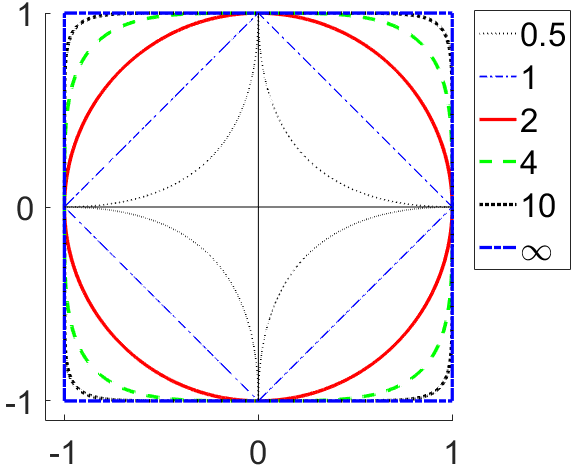
\includegraphics[width=0.25\columnwidth ]{UnitCircles.png}}
\caption{Unit level sets for $l_p$ functionals (``Unit spheres'').}
\label{fig:UnitCircles}
\end{figure}

Several different indicators were used to study concentration of distances:
\begin{itemize}
\item Relative contrast \cite{beyer1999, aggarwal2001, francois2007concentration}

\begin{equation}
\text{RC}_p(X,y)=\frac{|\max_i \|x_i-y\|_p - \min_i \|x_i-y\|_p|}{\min_i \|x_i-y\|_p}; \label{eq:RC}
\end{equation}
\item Coefficient of variations or relative variance \cite{demartines1994analyse, yianilos1999excluded, francois2007concentration}

\begin{equation}
\text{CV}_p(X,y)=\frac{\sqrt{var(\|x_i-y\|_p|)}}{mean(\|x_i-y\|_p)}, \label{eq:CV}
\end{equation}
where $var(x)$ is variance and $mean(x)$ is mean value of random variable $x$;
\item Hubness (popular nearest neighbours) \cite{radovanovic2010}.
\end{itemize}
In our study, we use RC and CV.

Table 2  in \cite{aggarwal2001}  shows that the proportion of cases where $\text{RC}_1>\text{RC}_2$ increases with dimension. It can be easily shown that for special choice of $X$ and $y$ all three relations are possible between RC$_1$ and RC$_2$: $\text{RC}_1(X,y)>\text{RC}_2(X,y)$ (all lines in Figure~\ref{fig:sets}, $\text{RC}_1(X,y)=\text{RC}_2(X,y)$, exclude row 6), or $\text{RC}_1(X,y)<\text{RC}_2(X,y)$ (row 6 in Figure~\ref{fig:sets}). To evaluate the probabilities of these three outcomes, we performed the following experiment. We generated $X$ dataset with $k$ points and $100$ coordinates. Each coordinate of each point was uniformly randomly generated in the interval $[0, 1]$. For each dimension $d=1, 2, 3, 4, 10, 15, 20, 100$ we create a $d$ dimensional database $X_d$ by selecting the first $d$ coordinates of points in $X$. We calculated $\text{RC}_p$ as the mean value of RC for each point in $X_d$:

\begin{equation*}
\text{RC}_p=\frac{1}{k}\sum_{i=1}^{k}\text{RC}_p(X_d\backslash \{x_i\},x_i),
\end{equation*}
where $X\backslash\{y\}$ is the $X$ database without the point $y$. We repeated this procedure 1000 times and calculated the fraction of cases when $\text{RC}_1>\text{RC}_2$. The results of this experiment are presented in Table~\ref{tab:RCComp}. Table~\ref{tab:RCComp} shows that for $k=10$ points our results are very similar to the results  presented in  Table 2 in \cite{aggarwal2001}. Increasing the number of points shows that even with a relatively small number of points ($k\approx 20$) for almost all databases $\text{RC}_1>\text{RC}_2$.

\begin{table}[tb]
\caption{Comparison of RC for $l_1$ and $l_2$ for different dimension of space (Dim) and different number of points}
\centering
\begin{tabular}{|c|c|c|c|c|}
\hline
\textbf{Dim}&\multicolumn{4}{|c|}{\textbf{$P(\text{RC}_2<\text{RC}_1)$ for \# of points}} \\
\cline{2-5}
 & \textbf{10 \cite{aggarwal2001}} & \textbf{10} & \textbf{20} & \textbf{100} \\
\hline
  1 & 0 & 0 & 0 & 0 \\ \hline
  2 & 0.850 & 0.850 & 0.960 & 1.00 \\ \hline
  3 & 0.887 & 0.930 & 0.996 & 1.00 \\ \hline
  4 & 0.913 & 0.973 & 0.996 & 1.00 \\ \hline
 10 & 0.956 & 0.994 & 1.00 & 1.00 \\ \hline
 15 & 0.961 & 1.000 & 1.00 & 1.00 \\ \hline
 20 & 0.971 & 0.999 & 1.00 & 1.00 \\ \hline
100 & 0.982 & 1.000 & 1.00 & 1.00 \\ \hline

\end{tabular}
\label{tab:RCComp}
\end{table}

This means that appearance of a significant proportion of cases when $\text{RC}_2>\text{RC}_1$ is caused by a very small sample size. For not so small samples, there is almost always $\text{RC}_2<\text{RC}_1$.
This is mainly because the pairs of nearest (farthest) points can be different for different metrics.
Several examples of such sets are presented in Figure~\ref{fig:sets}.
Figure~\ref{fig:sets} shows that $\text{RC}_2<\text{RC}_\infty$ in rows 3, 5, 6, and 8 and $\text{RC}_1<\text{RC}_2$ in row 6. These results allow us to formulate the hypothesis that in general case almost always $\text{RC}_p<\text{RC}_q, \forall p>q$. RC is widely used to study the properties of a finite set of points, but CV is more appropriate for point distributions. We hypothesise that $\text{CV}_p<\text{CV}_q, \forall p>q$.

\begin{figure}[p]
\centerline{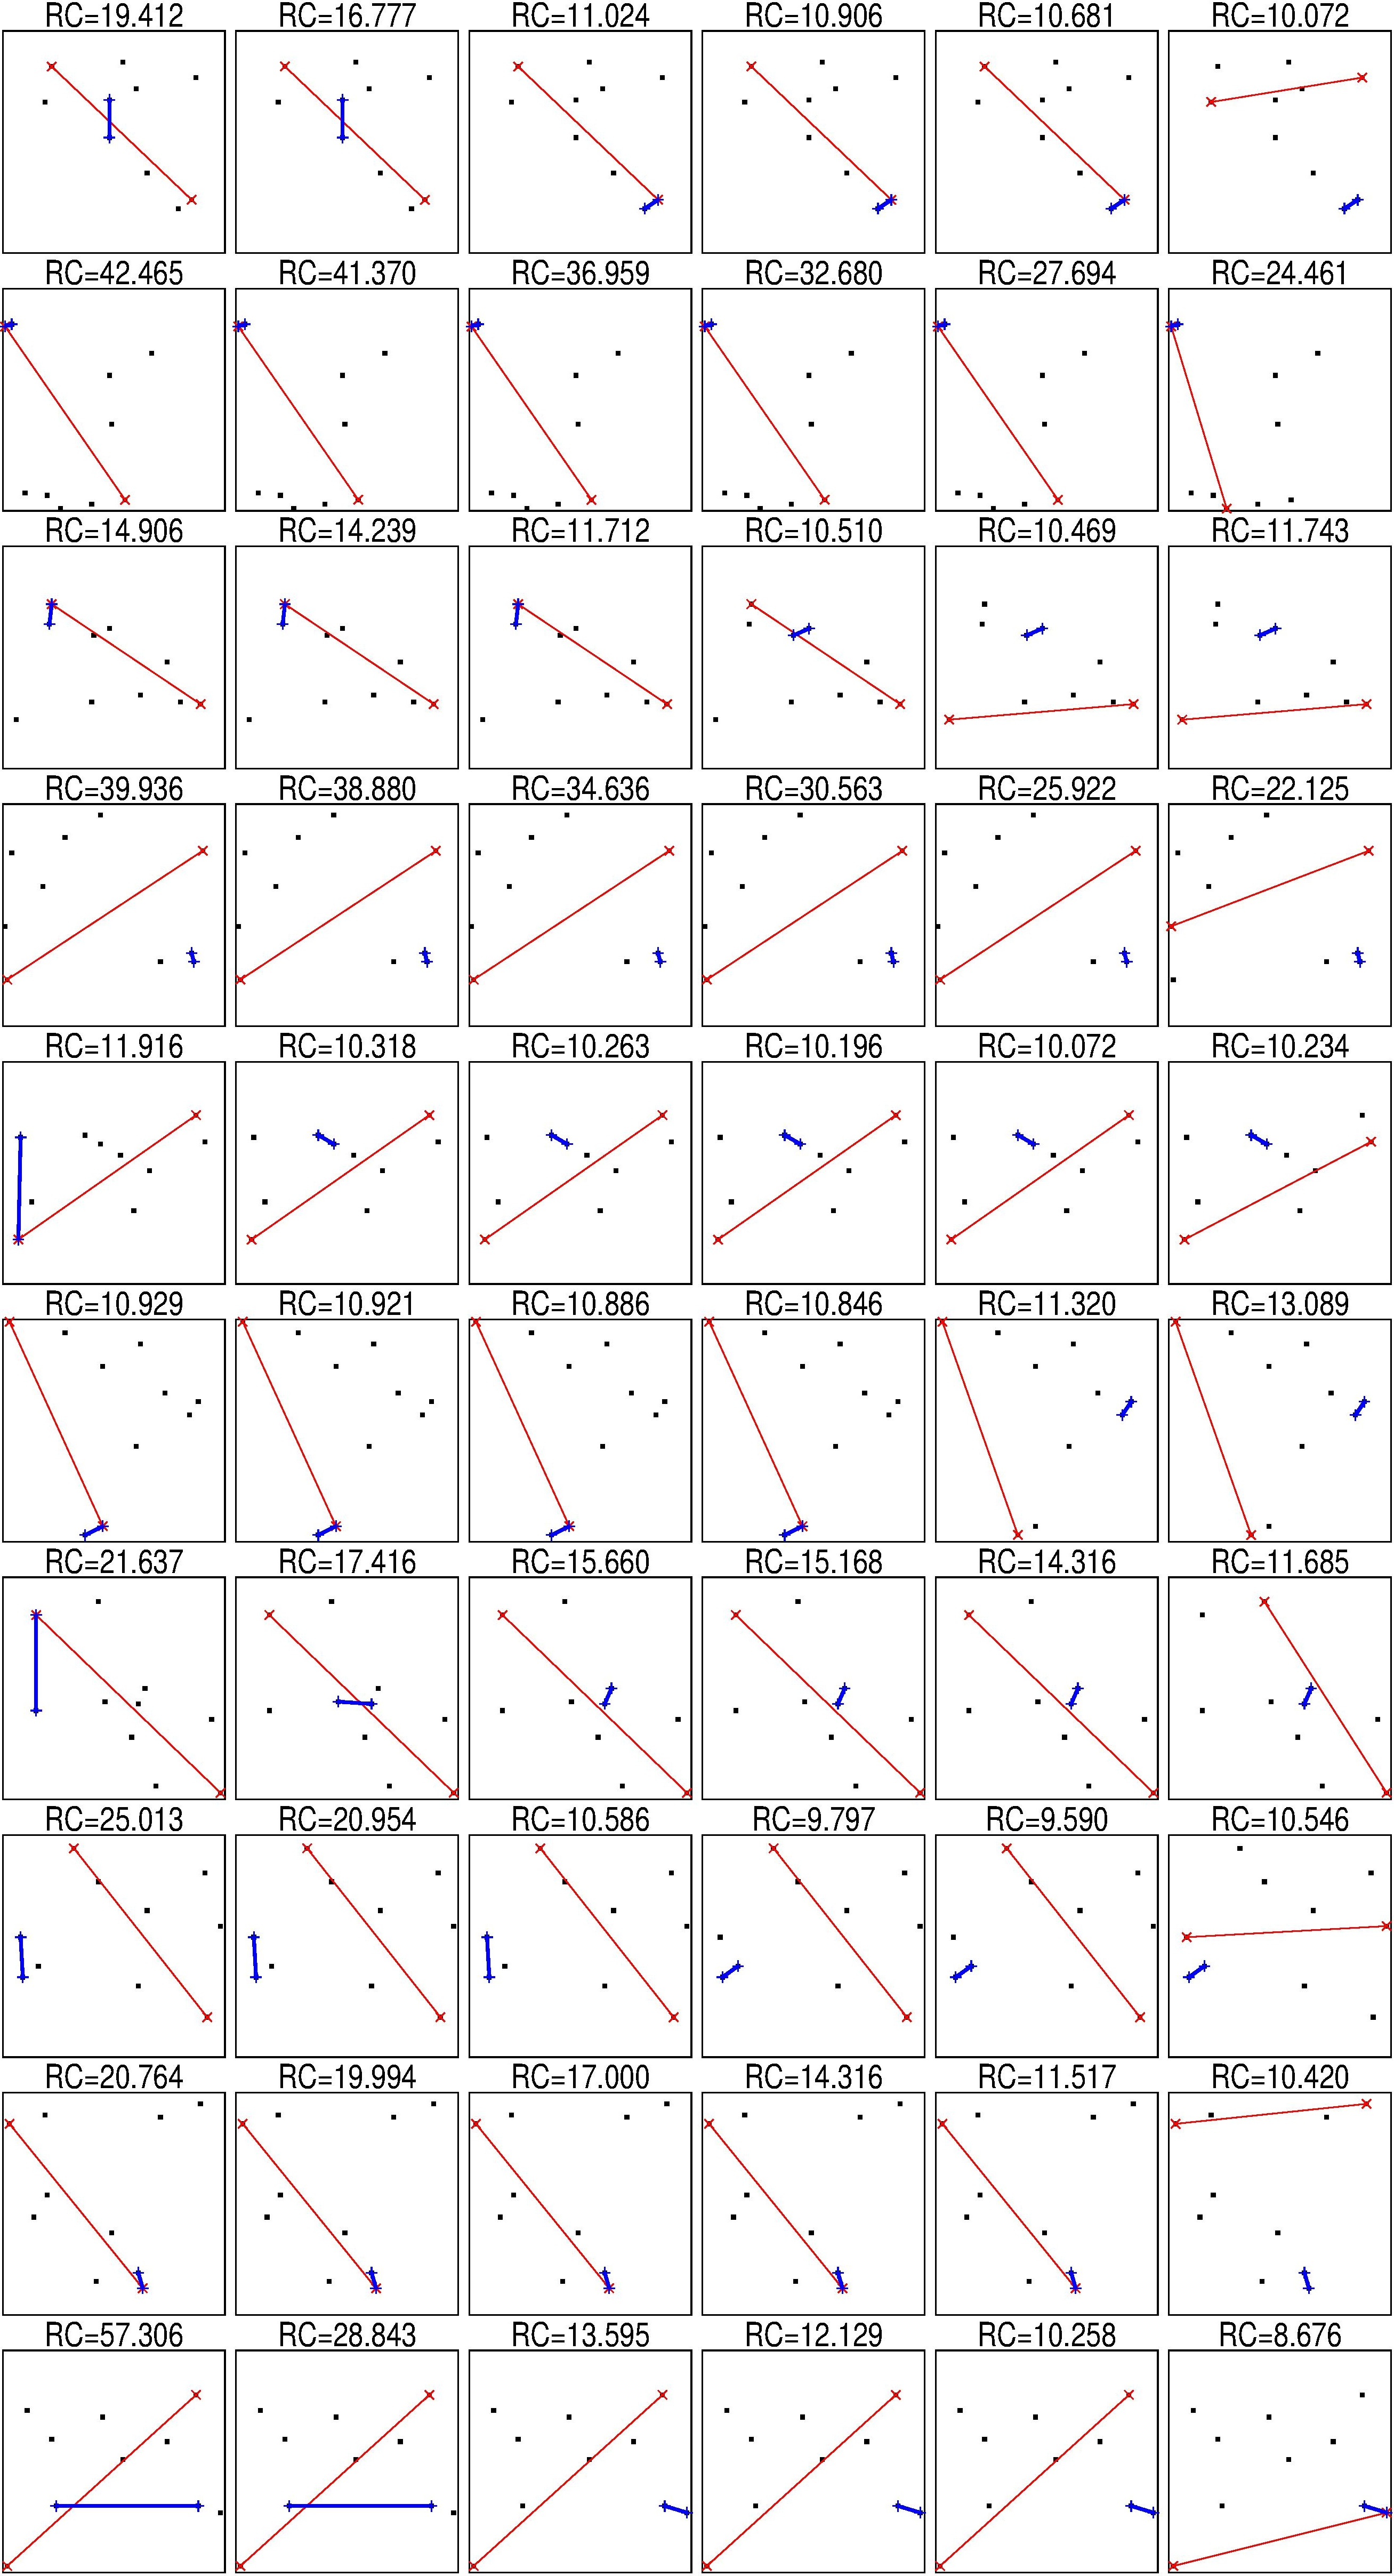
\includegraphics[width=0.7\columnwidth ]{ForTab2.png}}\caption{10 randomly generated sets of 10 points, thin red line connects the furthest points and bold blue line connects closest points, columns (from left to right) corresponds to $p=0.01, 0.1, 0.5, 1, 2, \infty $ }
\label{fig:sets}
\end{figure}

To check these hypotheses we performed the following experiment. We created a $X$ database with 10,000 points in 200 dimensional space. Each coordinate of each point was uniformly randomly generated in the interval $[0, 1]$. We chose the set of dimensions $d=1, 2, 3, 4, 5, 10, 15,\ldots, 195, 200$ and the set of $l_p$ functionals $l_{0.01}, l_{0.1}, l_{0.5}, l_{1}, l_{2}, l_{4}, l_{10}, l_{\infty}$. For each dimension $d$ we prepared the $X_d$ database as the set of the first $d$ coordinates of points in $X$ database. For each $X_d$ database and $l_p$ functional we calculate the set of all pairwise distances $D_{dp}$. Then we estimated the following values:

\begin{equation*}
\text{RC}_p=\frac{\max D_{dp} - \min D_{dp}}{\min D_{dp}}, \text{CV}_p=\frac{\sqrt{var(D_{dp})}}{mean(D_{dp})} .
\end{equation*}
The graphs $\text{RC}_p$ and $\text{CV}_p$ are presented in Figure~\ref{fig:RC1}. Figure~\ref{fig:RC1} shows that our hypotheses are true. We see that RC and CV as functions of dimension have qualitatively the same shape but in different scales: RC in the logarithmic scale.
The paper \cite{aggarwal2001} states that the qualitatively different behaviour of $\max_i \|x_i\|_p-\max_i \|x_i\|_p$ was observed for different $p$. We found qualitatively the same behavior for relative values (RC). The small quantitative difference $\text{RC}_p-\text{RC}_q$ increases for $ d $ from 1 to about 10 and decreases with a further increase in dimension. This means that there could be some preference for using lower values of $p$ but the fractional metrics do not provide a panacea for the curse of dimensionality. To analyse this hypothesis, we study the real live benchmarks in the Section~\ref{compar}.

\begin{figure}[tb]
\centerline{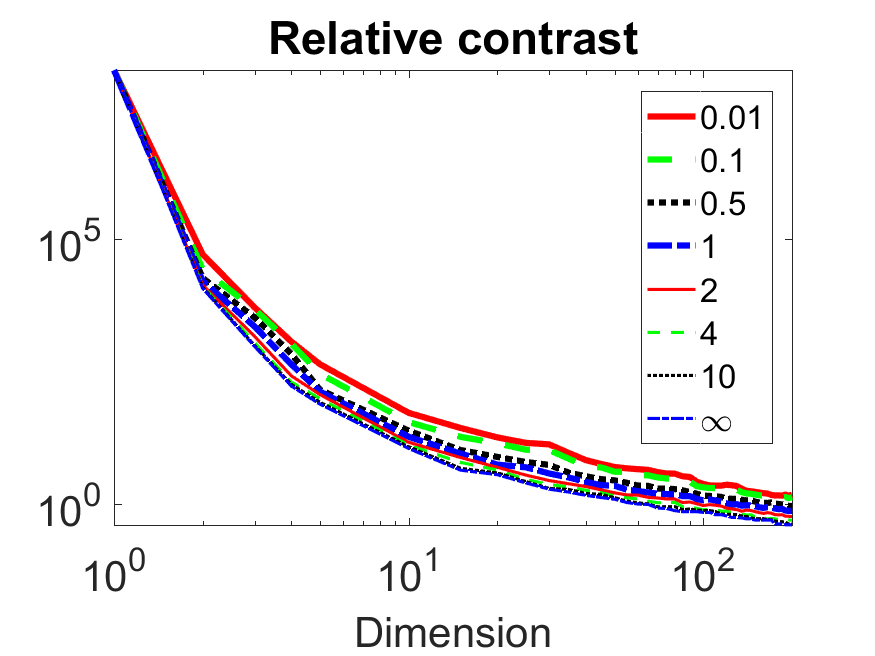
\includegraphics[width=0.4\columnwidth ]{RelCont1.png}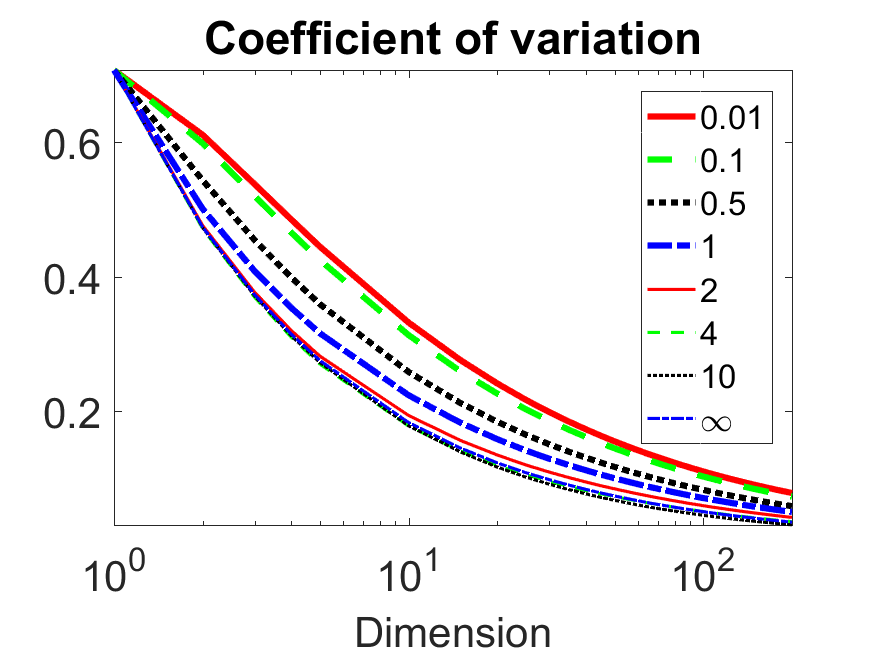
\includegraphics[width=0.4\columnwidth ]{CV1.png}}
\caption{Changes of RC (left) and CV (right) with dimension increasing for several metrics}
\label{fig:RC1}
\end{figure}

\section{Dimension estimation}\label{DimEst}
To consider high dimensional data and the curse or blessing of dimensionality, it is necessary to determine what dimensionality is. There are many different notions of data dimension. Evaluation of dimensionality become very important with emergence of many ``big data'' databases. The number of attributes is the dimension of the vector space or the Hamel dimension \cite{brown2012introduction} (hereinafter referred to as \#Attr). Fortunately, for the data mining tasks, the space dimension is not as important as the data dimension and the intrinsic data dimension is usually less than the dimension of space.
The concept of intrinsic, internal or effective data dimensionality is not well defined for the obvious reason: the data sets are finite and, therefore, the direct application of topological definitions of dimension gives zero.
The most popular approach to determining the data dimensionality is approximation of data sets by a continuous topological object. Perhaps, the first and at the same time widely used definition of intrinsic dimension is the dimension of the linear manifold of ``the best fit to data'' with sufficiently small deviations \cite{pearson1901}.
The simplest way to calculate such dimension is Principle Component Analysis (PCA) \cite{pearson1901, jobson2012applied}. Unfortunately, there are no unambiguous methods for determining the number of informative (important, relevant, etc.) principal components \cite{jackson1993stopping, ledesma2007determining, cangelosi2007component}. The two most widely used methods are the Kaiser rule \cite{guttman1954some, kaiser1960application} (hereinafter referred to as PCA-K) and the broken stick rule \cite{jackson1993stopping} (hereinafter referred to as PCA-BS).

Let us consider a $X$ database with $n$ data points $X={x_1,\ldots,x_n}$ and $d$ real-valued attributes, $x_i=(x_{i1},\ldots,x_{id})$.
Principal components are the eigenvalues of empirical covariance matrix $\Sigma(X)$. This matrix is symmetric and non-negative definite. This means that the eigenvalues of the $\Sigma(X)$ matrix are non-negative real numbers. Denote these values as $\lambda_1\ge\lambda_2\ge\cdots\ge\lambda_d$. The Fraction of Variance Explained (FVE) by $i$ principal component is $f_i=\frac{\lambda_i}{\sum_{j=1}^{d}\lambda_j}$.

The Kaiser rule states that all principal components with FVE greater or equal to the average FVE ($1/d$) are informative.

Consider a unit interval (stick) randomly broken into $d$ fragments. Let us numerate these fragments in descending order of their length: $s_1\ge s_2\ge\cdots\ge s_d$. Expected length of $i$ fragment is \cite{jackson1993stopping}

\begin{equation}\label{eq.BS}
b_i=\frac{1}{d}\sum_{j=i}^{d}\frac{1}{j}.
\end{equation}
The broken stick rule states that the first $k$ principal components are informative, where $k$ is the maximum number such that $f_i\ge b_i, \forall i\le k$.

In many problems, the empirical covariance matrix degenerates. Consider the projection of data on the first $k$ principal components: $\hat{X}=XV$, where the columns of the matrix $V$ are the first $k$ eigenvectors of the matrix $\Sigma(X)$. Eigenvalues of the empirical covariance matrix $\Sigma(\hat{X})$ are $\lambda_1,\lambda_2,\ldots,\lambda_k$. After the dimensionality reduction the condition number (the ratio of the lowest eigenvalue to the greatest) \cite{belsley2005regression} of the reduced covariance matrix should not be high in order to avoid the multicollinearity problem. The relevant definition \cite{gorban2018correction} of the intrinsic dimensionality refers directly to the condition number of the matrix $\Sigma(X)$: $k$ is the number of informative principal components if it is the smallest number such that

\begin{equation}\label{eq.CN}
\frac{\lambda_{k+1}}{\lambda_1}<\frac{1}{C},
\end{equation}
where $C$ is specified condition number, for example, $C=10$.  This approach is further referred to as PCA-CN. The PCA-CN intrinsic dimensionality is defined as the number of eigenvalues of the covariance matrix exceeding a fixed percent of its largest eigenvalue \cite{Fukunaga1971}.

The development of the idea of data approximation led to the appearance of principal manifolds \cite{gorban2008principal} and more sophisticated approximators, such as principal graphs and complexes \cite{gorban2007topological, gorban2010principal}. These approaches provide tools for evaluating the intrinsic dimensionality of data and measuring the data complexity \cite{zinovyev2013data}. Another approach uses complexes with vertices in data points: just connect the points with distance less than $\varepsilon$ for different $\varepsilon$ and get an object of combinatorial topology, simplicial complex \cite{Carlsson2009topology}. All these methods use an object embedded in the data space. They are called \emph{Injective Methods} \cite{bac2020lizard}. In addition, a family of \emph{Projective Methods} was developed. These methods do not construct a data approximator, but project the dataspace onto a space of lower dimension with preservation of similarity or dissimilarity of objects. A brief review of modern injective and projective methods can be found in \cite{bac2020lizard}.

Recent studies of curse/blessing dimensionality introduce a new method for evaluation intrinsic dimension: separability analysis. A detailed description of this method can be found in \cite{gorban2018correction, albergante2019estimating} (hereinafter referred to as SepD). For this study we used an implementation of separability analysis from \cite{matlabZin}. The main concept of this approach is the $\alpha$ Fisher separability: point $x$ of dataset $X$ is $\alpha$ Fisher separable from dataset $X$ if

\begin{equation}\label{eq.Sep}
(x,y)\le\alpha (x,x), \forall y\in X, y\ne x,
\end{equation}
where $(x,y)$ is dot product of vectors $x$ and $y$.

The last intrinsic dimension used in this study is the fractal dimension (hereinafter referred to as FracD). There are many versions of fractal dimension and we used R implementation from the RDimtools package \cite{RDimtools}. The considered definition of fractal dimension is
$$d_f=\lim_{r\to 0}\frac{\log(N(r))}{\log(1/r)},$$
where $r$ is the size of the $d$-cubic box in the regular grid and $N(r)$ is the number of cells with data points in this grid. Since the data set is finite the limit is substituted by slope of the linear regression without intercept.


\section{Comparison of $l_p$ functionals}\label{compar}

In Section~\ref{MesConc}, we demonstrated  that $\text{RC}_p$ is greater for smaller  $p$. It was shown in \cite{beyer1999} that greater RC means `more meaningful' task for KNN. We decided to compare different $l_p$ functions for KNN classification. Classification has one additional advantage over regression and clustering problems: classification quality measure is classifier independent and similarity measure independent \cite{sammut2011}.
For this study we selected three classification quality criteria: the Total Number of Neighbours of the Same Class (TNNSC), accuracy (fraction of correctly recognised cases), sum of sensitivity (fraction of correctly solved cases of positive class) and specificity (fraction of correctly solved cases of negative class). TNNSC is not an obvious indicator of classification quality and we use it for comparability of our results with \cite{aggarwal2001}. 11 nearest neighbours as the method of classification was selected also for comparability with \cite{aggarwal2001}.

\subsection{Databases for comparison}

We selected 25 databases from UCI Data repository \cite{Dua2017}. To select the databases, we applied the following criteria:
\begin{enumerate}
  \item Data are not time-series.
  \item Database is formed for the binary classification problem.
  \item Database does not contain any missing values.
  \item The number of attributes is less than the number of observations and is greater than 3.
  \item All predictors are binary or numeric.
\end{enumerate}

Totally, we selected 25 databases and 37 binary classification problems.
A total of 25 databases and 37 binary classification tasks were selected (some databases contain more than one classification problem).
For simplicity, we refer to each task as a `database'. The  list of selected databases is presented in Table~\ref{tab:DBs}.

\begin{table}[tb]
\caption{Databases selected for analysis}
\centering
\tablesize{\footnotesize} %% You can specify the fontsize here, e.g., \tablesize{\footnotesize}. If commented out \small will be used.
\begin{tabular}{lcrrrrrrr}
\toprule
\textbf{Name}& \textbf{Source}&\textbf{\#Attr.}&\textbf{Cases}&\textbf{PCA-K}&\textbf{PCA-BS}&\textbf{PCA-CN}&\textbf{SepD}&\textbf{FracD}\\
\hline
Blood & \cite{bloodDB} & 4 & 748 & 2 & 2 & 3 & 2.4 & 1.6\\ \hline
Banknote authentication & \cite{banknoteDB} & 4 & 1,372 & 2 & 2 & 3 & 2.6 & 1.9\\ \hline
Cryotherapy & \cite{khozeimeh2017, khozeimeh2017a, CryotherapyDB} & 6 & 90 & 3 & 0 & 6 & 4.1 & 2.5\\ \hline
Vertebral Column & \cite{VertebralDB} & 6 & 310 & 2 & 1 & 5 & 4.4 & 2.3\\ \hline
Immunotherapy & \cite{khozeimeh2017, khozeimeh2017a, ImmunotherapyDB} & 7 & 90 & 3 & 0 & 7 & 5.1 & 3.2\\ \hline
HTRU2 & \cite{HTRU2BD, HTRU2BD2, lyon2016} & 8 & 17,898 & 2 & 2 & 4 & 3.06 & 2.4\\ \hline
ILPD (Indian Liver &&&&&&&&\\
Patient Dataset) & \cite{ILDPDB} & 10 & 579 & 4 & 0 & 7 & 4.3 & 2.1\\ \hline
Planning Relax & \cite{RelaxDB} & 10 & 182 & 4 & 0 & 6 & 6.09 & 3.6\\ \hline
MAGIC Gamma Telescope & \cite{TelescopeDB} & 10 & 19,020 & 3 & 1 & 6 & 4.6 & 2.9\\ \hline
EEG Eye State & \cite{EEGDB} & 14 & 14,980 & 4 & 4 & 5 & 2.1 & 1.2\\ \hline
Climate Model Simulation &&&&&&&&\\
Crashes & \cite{ClimateDB} & 18 & 540 & 10 & 0 & 18 & 16.8 & 21.7\\ \hline
Diabetic Retinopathy Debrecen & \cite{DiabeticDB, antal2014} & 19 & 1,151 & 5 & 3 & 8 & 4.3 & 2.3\\ \hline
SPECT Heart & \cite{HeartDB} & 22 & 267 & 7 & 3 & 12 & 4.9 & 11.5\\ \hline
Breast Cancer  & \cite{BreastDB} & 30 & 569 & 6 & 3 & 5 & 4.3 & 3.5\\ \hline
Ionosphere & \cite{IonosphereDB} & 34 & 351 & 8 & 4 & 9 & 3.9 & 3.5\\ \hline
QSAR biodegradation & \cite{mansouri2013, QSARDB} & 41 & 1,055 & 11 & 6 & 15 & 5.4 & 3.1\\ \hline
SPECTF Heart & \cite{HeartDB} & 44 & 267 & 10 & 3 & 6 & 5.6 & 7\\ \hline
MiniBooNE particle &&&&&&&&\\
identification & \cite{MiniBooNEDB} & 50 & 130,064 & 4 & 1 & 1 & 0.5 & 2.7\\ \hline
First-order theorem proving &&&&&&&&\\
 (6 tasks) & \cite{bridge2014, TheoremDB} & 51 & 6,118 & 13 & 7 & 9 & 3.4 & 2.04\\ \hline
Connectionist Bench (Sonar) & \cite{SonarDB} & 60 & 208 & 13 & 6 & 11 & 6.1 & 5.5\\ \hline
Quality Assessment of &&&&&&&&\\
Digital Colposcopies (7 tasks) & \cite{ColposcopiesDB, fernandes2017} & 62 & 287 & 11 & 6 & 9 & 5.6 & 4.7\\ \hline
LFW & \cite{LFWTech} & 128 & 13,233 & 51 & 55 & 57 & 13.8 & 19.3\\ \hline
Musk 1 & \cite{MuskDB} & 166 & 476 & 23 & 9 & 7 & 4.1 & 4.4\\ \hline
Musk 2 & \cite{MuskDB} & 166 & 6,598 & 25 & 13 & 6 & 4.1 & 7.8\\ \hline
Madelon & \cite{guyon2005, MadelonDB} & 500 & 2,600 & 224 & 0 & 362 & 436.3 & 13.5\\ \hline
Gisette & \cite{GisetteDB, guyon2005} & 5,000 & 7,000 & 1465 & 133 & 25 & 10.2 & 2.04\\
\bottomrule
\end{tabular}
\label{tab:DBs}
\end{table}

We do not set out to determine the best database preprocessing for each database. We just use three preprocessing for each database:
\begin{itemize}
  \item empty preprocessing means usage data `as is';
  \item standardisation means shifting and scaling data to have a zero mean and unit variance;
  \item min-max normalization refers to shifting and scaling data in the interval $[0,1]$.
\end{itemize}


\subsection{Approaches to comparison}

Our purpose is to compare $l_p$ functionals but not to create the best classifier for each  problem. Following \cite{aggarwal2001}, we use the 11NN  classifier. One of the reasons for choosing KNN is strong dependence of KNN on used metrics and, on the other hand, the absence of any assumption about the data, excluding the principle: tell me your neighbours, and I will tell you what you are. In our study we consider 11NN with $l_{0.01}, l_{0.1}, l_{0.5}, l_1, l_2, l_4, l_{10}, l_\infty$ as different algorithms.
We applied the following indicators to compare 11NN classifiers (algorithms) for listed $l_p$ functionals:
\begin{itemize}
  \item the number of databases for which the algorithm is the best \cite{demvsar2006statistical};
  \item the number of databases for which the algorithm is the worst \cite{demvsar2006statistical};
  \item the number of databases for which the algorithm has performance that is statistically insignificantly different from the best;
  \item the number of databases for which the algorithm has performance that is statistically insignificantly different from the worst;
  \item the Friedman test \cite{friedman1940comparison}, \cite{friedman1937use} and post hoc Nemenyi test \cite{nemenyi1962distribution} which were specially developed to compare multiple algorithms;
  \item the Wilcoxon signed rank test was used to compare three pairs of metrics.
\end{itemize}

The first four approaches we call frequency comparison. To avoid discrepancies, a description of all used statistical tests is presented below.

\subsubsection{Proportion estimation}
Since two measures of classification quality - accuracy and $\text{TNNSC}/(11\times n)$, where $n$ is the number of cases in the database - are proportions, we can apply z-test for proportion estimations \cite{altman2013statistics}. We want to compare two proportions with the same sample size, so we can use a simplified formula for test statistics:

\begin{equation*}
z=\frac{|p_1 - p_2|}{\sqrt{\frac{p_1+p_2}{n}\big(1-\frac{p_1+p_2}{2}\big)}},
\end{equation*}
where $p_1$ and $p_2$ are two proportions for comparison. \emph{P}-value of this test is probability of observing by chance the same or greater $z$ if both samples are taken from the same population. \emph{P}-value is $p_z=\Phi(-z)$, where $\Phi(z)$ is the standard cumulative normal distribution.
There is a problem of reasonable choice of significance level. The selected databases contain from 90 to 130,064 cases. Using the same threshold for all databases is meaningless \cite{biau2008statistics, kadam2010sample}. The required sample size $n$ can be estimated through the specified significance level of $1-\alpha$, the statistical power $1-\beta$, the expected effect size $e$, and the population variance $s^2$. For the  normal distribution (since we use z-test) this estimation is:

\begin{equation*}
n=\frac{2(z_{1-\alpha}+z_{1-\beta})^2s^2}{e^2}.
\end{equation*}
In this study, we assume that the significance level is equal to the statistical power $\alpha=\beta$, the expected effect size is 1\% (1\% difference in accuracy is large enough), and the  population variance can be estimated by the formula

\begin{equation*}
s^2=n\frac{n_+}{n}\big(1-\frac{n_+}{n}\big)=\frac{n_+(n-n_+)}{n},
\end{equation*}
where $n_+$ is the number of cases in the positive class. Based on this assumption, we can estimate a reasonable level of significance as

\begin{equation*}
\alpha=\Phi\left(\frac{e}{s}\sqrt{\frac{n}{8}} \right).
\end{equation*}
Usage of eight $l_p$ functionals means multiple testing. To avoid overdetection problem we apply Bonferroni correction \cite{bonferroni1935calcolo}. On the other hand, usage of too high significance level is also meaningless \cite{biau2008statistics}. As a result we select the significance level as

\begin{equation*}
\alpha=\max \bigg \{\frac{1}{28}\Phi\bigg(\frac{e}{s}\sqrt{\frac{n}{8}} \bigg),0.00001\bigg \} .
\end{equation*}
The difference between two proportions (TNNSC or accuracy) is statistically significant if $p_z<\alpha$.
It must be emphasized that for TNNSC the number of cases is $11n$ because we consider 11 neighbours for each point.

\subsubsection{Friedman test and post hoc Nemenyi test}
One of the widely used statistical tests for comparing algorithms on many databases is the Friedman test \cite{friedman1940comparison, friedman1937use}. To apply this test, we firstly need to apply the tied ranking for the classification quality score for one database: if several classifiers provide exactly the same quality score then the rank of all such classifiers will be equal to the average value of the ranks for which they were tied \cite{friedman1937use}. Let us denote the number of used databases as $N$, the number of used classifiers as $m$ and the rank of classifier $i$ for database $j$ as $r_{ji}$. The mean rank of classifier $i$ is

\begin{equation*}
R_i=\frac{1}{N}\sum_{j=1}^{N} r_{ji}.
\end{equation*}
Test statistics is

\begin{equation*}
\chi^2_F=\frac{N^2(m-1)\Big(4\sum_{i=1}^{m} R_{i}^2 -m(m+1)^2\Big)}{4\sum_{i=1}^{m}\sum_{j=1}^{N} r_{ji}^2 -Nm(m+1)^2}.
\end{equation*}
Test statistics under null hypothesis that all classifiers have the same performance follows the $\chi^2$ distribution with $m-1$ degrees of freedom. \emph{P}-value of this test is the probability of observing by chance the same or greater $\chi^2_F$ if all classifiers have the same performance. \emph{P}-value is $p_\chi=1-F(\chi^2_F; m-1)$, where $F(\chi; df)$ is the cumulative $\chi^2$ distribution with $df$ degrees of freedom. Since we only have 37 databases, we decide to use the 95\% significance level.

If the Friedman test shows enough evidence to reject null hypothesis, then we can conclude that not all classifiers have the same performance. To identify pairs of classifiers with significantly different performances we applied the post hoc Nemenyi test \cite{nemenyi1962distribution}. Test statistics for comparing of classifiers $i$ and $j$ is $|R_i-R_j|$. To identify pairs with statistically significant differences the critical distance

\begin{equation*}
\text{CD}=q_{\alpha m} \sqrt{\frac{m(m+1)}{6N}}.
\end{equation*}
is used. $q_{\alpha m}$ is critical value for Nemenyi test with significance level of $1-\alpha$ and $m$ degrees of freedom. The difference of classifiers performances is statistically significant with significance level of $1-\alpha$ if $|R_i-R_j|>CD$.

\subsubsection{Wilcoxon signed rank test}
To compare the performance of two classifiers on several databases we applied the Wilcoxon signed rank test \cite{wilcoxon1945individual}. For this test we used standard Matlab function \textbf{signrank} \cite{matlabWilcoxon}.

%%%%%%%%%%%%%%%%%%%%%%%%%%%%%%%%%%%%%%%%%%
\section{Dimension comparison}\label{DimComp}

An evaluation of six dimensions (number of attributes (dimension of space) and five intrinsic dimensions of data) for benchmarks is presented in Table~\ref{tab:DBs}. It can be seen that for each considered intrinsic dimension of data this dimension does not grow monotonously with the number of attributes for the given set of benchmarks. The correlation matrix of all six dimensions is presented in Table~\ref{tab:CorrDist}. There are two groups of highly correlated dimensions:
\begin{itemize}
\item \#Attr, PCA-K and PCA-BS;
\item PCA-CN and SepD.
\end{itemize}
Correlations between groups are low (the maximum value is 0.154). The fractal dimension (FracD) is correlated (but is not strongly correlated) with PCA-CN and SepD.

\begin{table}[b]
\caption{Correlation matrix for six dimensionality: two groups of highly correlated dimensions are highlighted by the background colours}
\centering
%\scriptsize
\begin{tabular}{|l|r|r|r|r|r|r|r|}
\hline
\textbf{Dimension}&\textbf{\#Attr}&\textbf{PCA-K}&\textbf{PCA-BS}&\textbf{PCA-CN}&\textbf{SepD}&\textbf{FracD}\\\hline

\#Attr&\cellcolor{blue!30}{1.000}&\cellcolor{blue!30}{0.998}&\cellcolor{blue!30}{0.923}&0.098&0.065&-0.081\\ \hline
PCA-K&\cellcolor{blue!30}{0.998}&\cellcolor{blue!30}{1.000}&\cellcolor{blue!30}{0.917}&0.154&0.119&-0.057\\ \hline
PCA-BS&\cellcolor{blue!30}{0.923}&\cellcolor{blue!30}{0.917}&\cellcolor{blue!30}{1.000}&0.018&-0.058&0.075\\ \hline
PCA-CN&0.098&0.154&0.018&\cellcolor{green!30}{1.000}&\cellcolor{green!30}{0.992}&0.405\\ \hline
SepD&0.065&0.119&-0.058&\cellcolor{green!30}{0.992}&\cellcolor{green!30}{1.000}&0.343\\ \hline
FracD&-0.081&-0.057&0.075&0.405&0.343&1.000\\ \hline

\end{tabular}
\label{tab:CorrDist}
\end{table}

Consider the first group of correlated dimensions. Linear regressions of PCA-K and PCA-BS on \#Attr are

\begin{equation*}\label{eq.LinRegK}
\begin{split}
\text{PCA-K} &= 0.29 \text{\#Attr},\\
\text{PCA-BS} &= 0.027 \text{\#Attr}.
\end{split}
\end{equation*}

It is necessary to emphasize that a coefficient 0.29 (0.027 for PCA-BS) was determined only for datasets considered in this study and can be different for another datasets, but multiple R squared equals 0.998 (0.855 for PCA-BS), shows that this dependence is not accidental. What is the reason for so strong correlations of these dimensions? It can be shown, that these dimensions are sensitive to irrelevant or redundant attributes. The simplest example is adding of highly correlated attributes. To illustrate this property of these dimensions, consider an abstract database $X$ with $d$ standardised attributes and a covariance matrix $\Sigma$. This covariance matrix has $d$ eigenvalues $\lambda_1\ge\lambda_2\ge\ldots\ge\lambda_d$ and corresponding eigenvectors $v_1,\ldots,v_d$. To determine the PCA-K dimension we must compare FVE of each principal component with the threshold $1/d$. Since all attributes are standardized, the elements of the main diagonal of the matrix $\Sigma$ are equal to one. This mean that $\sum_{i=1}^{d}\lambda_i=d$ and the FVE of $i$ principal component is $f_i=\frac{\lambda_i}{\sum_{j=1}^{d}\lambda_j}=\lambda_i/d$.

Consider duplication of attributes: add copies of the original attributes to the data table. This operation does not add any information to the data and, in principle, should not affect the intrinsic dimension of the data for any reasonable definition.

Denote all object for this new database by superscript $(1)$. New dataset is $X^{(1)}=X|X$, where symbol $|$ denotes the concatenation of two row vectors. For any data vectors $x^{(1)}$ and $y^{(1)}$ the dot product is $(x^{(1)}, y^{(1)})=2(x, y)$.

For a new dataset $X^{(1)}$ the covariance matrix has the form
\begin{equation*}\label{eq.Covar}
\Sigma ^{(1)}= \begin{bmatrix}
\Sigma & \Sigma\\
\Sigma & \Sigma
\end{bmatrix}.
\end{equation*}
The first $d$ eigenvectors can be represented as $v^{(1)}_i=(v_i^\intercal |v_i^\intercal)^\intercal$, where $\intercal$ means transposition of the matrix (vector). Calculate the product of $v^{(1)}_i$ and $\Sigma ^{(1)}$:

\begin{equation*}\label{eq.Eigen}
%\begin{split}
\Sigma ^{(1)}v^{(1)}_i= \begin{bmatrix}
\Sigma & \Sigma\\
\Sigma & \Sigma
\end{bmatrix}
\begin{pmatrix}
v_i \\
v_i
\end{pmatrix}
%&
=
\begin{pmatrix}
\Sigma v_i + \Sigma v_i \\
\Sigma v_i + \Sigma v_i
\end{pmatrix}\\=
\begin{pmatrix}
\lambda_iv_i + \lambda_iv_i \\
\lambda_iv_i + \lambda_iv_i
\end{pmatrix}
%&
=2\lambda_i
\begin{pmatrix}
v_i\\
v_i
\end{pmatrix}=
2\lambda_iv_i^{(1)}.
%\end{split}
\end{equation*}
As we can see, each of the first $d$ eigenvalues become twice as large ($\lambda^{(1)}_i=2\lambda_i, \forall i\le d$). This means that the FVE of the first $d$ principal components have the same values
\begin{equation*}
f_i^{(1)}=\frac{\lambda^{(1)}_i}{2d}=\frac{2\lambda_i}{2d}=\frac{\lambda_i}{d}=f_i, \forall i\le d.
\end{equation*}
Since sum of the eigenvalues of the matrix $\Sigma ^{(1)}$ is $2d$ we can conclude that $\lambda^{(1)}_i=0, \forall i>d$. We can repeat the described procedure for copying attributes several times and determine the values $\lambda^{(m)}_i=m\lambda_i, f_i^{(m)}=f_i \forall i\le d$ and $\lambda^{(m)}_i=0, \forall i>d$, where $m$ is the number of copies of attributes added. For the database $X^{(m)}$, the informativeness threshold of principal components is $\frac{1}{md}$. Obviously, for any nonzero eigenvalue $\lambda_i>0$ there exists $m$ such that $\lambda_i>\frac{1}{(m+1)d}$. This means that trivial operation of adding copies of attributes can increase informativeness of principal components and the number of informative main components or PCA-K dimension.

To evaluate the effect of the attribute copying procedure on the broken stick dimension, the following two propositions are needed:
\begin{Proposition}\label{prop1}
If $d=2k$, then $b^{(1)}_{k+s}>b_{k+s}, s=1,\ldots,k$ and $b^{(1)}_{k-s}<b_{k-s}, s=0,\ldots, k-1$.
\end{Proposition}

\begin{Proposition}\label{prop2}
If $d=2k+1$, then $b^{(1)}_{k+s}>b_{k+s}, s=2,\ldots,k+1$ and $b^{(1)}_{k-s}<b_{k-s}, s=-1,\ldots,k-1$.
\end{Proposition}

Proofs of these propositions are presented in Appendix~\ref{PropProof}.

The simulation results of process of the attribute copying for `Musk 1' and `Gisette' databases are presented in Table~\ref{tab:DuplDist}.

\begin{table}[t]
\caption{Attribute duplication process for `Musk 1' and `Gisette' databases}
\centering
%\scriptsize
\begin{tabular}{r|rrr|rrr}
\toprule

&\multicolumn{3}{|c|}{\textbf{Musk}}&\multicolumn{3}{c|}{\textbf{Gizette}}\\ \cline{2-7}
\textbf{m}&\textbf{\#Attr}&\textbf{PCA-K}&\textbf{PCA-BS}&\textbf{\#Attr}&\textbf{PCA-K}&\textbf{PCA-BS}\\
\midrule
0&166&23&9&4,971&1,456&131\\
1&332&34&16&9,942&2,320&1,565\\
2&498&40&23&14,913&2,721&1,976\\
3&664&45&28&19,884&2,959&2,217\\
4&830&49&32&24,855&3,122&2,389\\
5&996&53&33&29,826&3,242&2,523\\
10&1,826&63&39&54,681&3,594&2,909\\
50&8,466&94&62&253,521&4,328&3,641\\
100&16,766&109&73&502,071&4,567&3,926\\
500&83,166&139&102&2,490,471&4,847&4,491\\
1,000&166,166&150&115&4,975,971&4,863&4,664\\
5,000&830,166&163&141&24,859,971&4,865&4,852\\
10,000&1,660,166&166&151&49,714,971&4,866&4,863\\
\bottomrule

\end{tabular}
\label{tab:DuplDist}
\end{table}

Now we are ready to evaluate the effect of duplication of attributes on the dimensions under consideration, keeping in mind that nothing should change for reasonable definitions of data dimension.
\begin{itemize}
  \item The dimension of the vector space of the dataset $X^{(m)}$ is $(m+1)d$ (see Table~\ref{tab:DuplDist}).
  \item For the dimension defined by the Kaiser rule PCA-K, the threshold of informativeness is $1/(m+1)d$. This means that for all principal components with nonzero eigenvalues, we can take large enough $m$ to ensure that these principal components are ``informative'' (see Table~\ref{tab:DuplDist}). The significance threshold decreases linearly with increasing $m$.
  \item For the dimension defined by the broken stick rule PCA-BS, we observe initially an increase in the thresholds for the last half of the original principal components, but then the thresholds $b^{(m)}_i$ decrease with an increase in $m$ for all $i\le d$. This means that for all principal components with nonzero eigenvalues, we can take large enough $m$ to ensure that these principal components are ``informative''  (see Table~\ref{tab:DuplDist}). The thresholds of significance decrease non-linearly with increasing $m$. This slower than linear thresholds decreasing shows that PCA-BS is less sensitivity to irrelevant attributes than \#Attr or PCA-K.
  \item For the PCA-CN dimension defined by condition number, nothing changes in the described procedure since simultaneous multiplying of all eigenvalues by a nonzero constant does not change the fraction of eigenvalues in the condition~\eqref{eq.CN}.
  \item Adding irrelevant objects does not change anything for separability dimension SepD, since the dot product of any two data points in the extended database is the dot products of the corresponding vectors in the original data set multiplied by $m+1$. This means that described extension of dataset change nothing in the separability inequality \eqref{eq.Sep}.
  \item There are no changes for the fractal dimension FracD, since the described extension of dataset do not change relative location of data points in space. This means that values $N(r)$ will be the same for original and extended datasets.
\end{itemize}



The second group of correlated dimensions includes PCA-CN, SepD, and FracD. The first two are extremely correlated and the last one is moderately correlated with the first two. Linear regressions of these dimensions are

\begin{equation*}
\begin{split}
\text{SepD} &= 1.17 \text{PCA-CN},\\
\text{FracD} &= 0.052 \text{PCA-CN}.
\end{split}
\end{equation*}

High correlation of these three dimensions requires additional investigations.

\section{Results of $l_p$ functionals comparison}
The results of a direct comparison of the algorithms are presented in Table~\ref{tab:BestWorst}. Table~\ref{tab:BestWorst} shows that `The best' indicator is not reliable and cannot be considered as a good tool for performance comparison \cite{demvsar2006statistical}. For example, for TNNSC with empty preprocessing, $l_{0.1}$ is the best for 11 databases and this is maximal value, but $l_{0.5}, l_1$ and $l_2$ are essentially better if we consider indicator `Insignificantly different from the best': 26 databases for $l_{0.1}$ and 31 databases for $l_{0.5}, l_1$ and $l_2$. This fact confirms that the indicator `Insignificantly different from the best' is more reliable. Unfortunately we cannot estimate this indicator for `sensitivity plus specificity' quality measure. Analysis of Table~\ref{tab:BestWorst} shows that on average $l_{0.5}, l_1, l_2$ and $l_4$ are the best and $l_{0.01}$ and $l_\infty$ are the worst.

\begin{table}[tb]
\caption{Frequency comparison for TNNSC, accuracy and sensitivity plus specificity}
\centering
\begin{tabular}{|l|r|r|r|r|r|r|r|r|}
\hline
\textbf{Indicator\textbackslash p for $l_p$ functional}&\textbf{0.01}&\textbf{0.1}&\textbf{0.5}&\textbf{1}&\textbf{2}&\textbf{4}&\textbf{10}&$\infty$\\
\hline
\multicolumn{9}{|c|}{\textbf{TNNSC}}\\ \hline
\multicolumn{9}{|c|}{Empty preprocessing}\\ \hline
The best & 2 & 11 & 5 & 10 & 7 & 1 & 1 & 1\\ \hline
Insignificantly different from the best & 17 & 26 & 31 & 31 & 31 & 30 & 23 & 22\\ \hline
The worst & 19 & 0 & 1 & 0 & 1 & 3 & 4 & 8\\ \hline
Insignificantly different from the worst & 34 & 23 & 17 & 19 & 21 & 21 & 25 & 29\\ \hline
\multicolumn{9}{|c|}{Standardisation}\\ \hline
The best & 0 & 5 & 10 & 11 & 6 & 2 & 1 & 1\\ \hline
Insignificantly different from the best & 19 & 26 & 33 & 32 & 31 & 30 & 25 & 24\\ \hline
The worst & 18 & 2 & 0 & 0 & 1 & 2 & 4 & 10\\ \hline
Insignificantly different from the worst & 35 & 24 & 20 & 19 & 20 & 21 & 25 & 28\\ \hline
\multicolumn{9}{|c|}{Min-max normalization}\\ \hline
The best & 1 & 5 & 10 & 13 & 4 & 6 & 1 & 3\\ \hline
Insignificantly different from the best & 19 & 26 & 32 & 31 & 30 & 29 & 26 & 26\\ \hline
The worst & 23 & 4 & 2 & 2 & 3 & 3 & 4 & 7\\ \hline
Insignificantly different from the worst & 36 & 24 & 22 & 21 & 22 & 22 & 26 & 26\\ \hline
\multicolumn{9}{|c|}{\textbf{Accuracy}}\\ \hline
\multicolumn{9}{|c|}{Empty preprocessing}\\ \hline
The best & 3 & 9 & 9 & 15 & 6 & 5 & 1 & 2\\ \hline
Insignificantly different from the best & 29 & 31 & 34 & 35 & 35 & 35 & 33 & 30\\ \hline
The worst & 13 & 3 & 1 & 2 & 4 & 4 & 9 & 14\\ \hline
Insignificantly different from the worst & 35 & 32 & 28 & 28 & 29 & 29 & 30 & 31\\ \hline
\multicolumn{9}{|c|}{Standardisation}\\ \hline
The best & 2 & 5 & 12 & 18 & 7 & 3 & 1 & 1\\ \hline
Insignificantly different from the best & 30 & 31 & 34 & 34 & 33 & 31 & 32 & 30\\ \hline
The worst & 13 & 4 & 0 & 0 & 2 & 6 & 7 & 13\\ \hline
Insignificantly different from the worst & 35 & 32 & 29 & 29 & 30 & 31 & 33 & 33\\ \hline
\multicolumn{9}{|c|}{Min-max normalization}\\ \hline
The best & 2 & 7 & 15 & 8 & 8 & 3 & 3 & 6\\ \hline
Insignificantly different from the best & 30 & 31 & 34 & 33 & 33 & 32 & 31 & 32\\ \hline
The worst & 18 & 6 & 3 & 4 & 5 & 9 & 8 & 8\\ \hline
Insignificantly different from the worst & 36 & 33 & 31 & 31 & 31 & 32 & 33 & 32\\ \hline

\multicolumn{9}{|c|}{\textbf{Sensitivity plus specificity}}\\ \hline
\multicolumn{9}{|c|}{Empty preprocessing}\\ \hline
The best & 4 & 8 & 7 & 12 & 7 & 5 & 1 & 1\\ \hline
The worst & 14 & 2 & 1 & 1 & 3 & 5 & 8 & 12\\ \hline
\multicolumn{9}{|c|}{Standardisation}\\ \hline
The best & 4 & 7 & 8 & 15 & 7 & 2 & 1 & 0\\ \hline
The worst & 13 & 3 & 0 & 0 & 2 & 5 & 4 & 15\\ \hline
\multicolumn{9}{|c|}{Min-max normalization}\\ \hline
The best & 5 & 8 & 13 & 6 & 9 & 3 & 4 & 5\\ \hline
The worst & 15 & 4 & 2 & 3 & 3 & 7 & 8 & 13\\ \hline

\end{tabular}
\label{tab:BestWorst}
\end{table}

The results of the Friedman and post hoc Nemenyi tests are presented in Table~\ref{tab:TestResults}. We applied these tests for three different preprocessings and three classification quality indicators. In total, we tested nine sets for eight algorithms and 37 databases. The post hoc Nemenyi test was used to define algorithms with performance that do not significantly differ from the best algorithm.
It can be seen that $l_{1}$ is the best for 6 of 9 sets and $l_{0.5}$ is the best for the remaining 3 sets. On the other hand, performances of $l_{0.5}, l_1$ and $l_2$ are insignificantly different from the best for all nine sets.

\begin{table}[tb]
\caption{Results of the Friedman test and post hoc Nemenyi test}
\centering
\begin{tabular}{|l|c|c|r|r|r|r|r|r|r|r|r|r|}
\hline
\textbf{Preprocessing}&\textbf{Quality}&\textbf{Friedman's}& \multicolumn{2}{|c|}{\textbf{The best $l_p$}}&\multicolumn{8}{|c|}{\textbf{Set of insignificantly different from the best}}
\\ \cline{4-13}
&\textbf{measure}&\textbf{\emph{p}-value}&\multicolumn{1}{|c|}{\textbf{$p$}}&\multicolumn{1}{|c|}{\textbf{$R_i$}}&\textbf{0.01}&\textbf{0.1}&\textbf{0.5}&\textbf{1}&\textbf{2}&\textbf{4}&\textbf{10}&$\infty$\\
\hline

 & TNNSC & $<0.0001$ & 1 & 6.2639 &  & X & X & X & X & X &  & \\ \cline{2-13}
Empty & Accuracy & $<0.0001$ & 1 & 6.2639 &  & X & X & X & X &  &  & \\ \cline{2-13}
 & Se+Sp & $<0.0001$ & 0.5 & 6.0556 &  & X & X & X & X &  &  & \\ \hline
 & TNNSC & $<0.0001$ & 1 & 6.6944 &  &  & X & X & X &  &  & \\ \cline{2-13}
Standardisation & Accuracy & $<0.0001$ & 1 & 6.8056 &  &  & X & X & X &  &  & \\ \cline{2-13}
 & Se+Sp & $<0.0001$ & 1 & 6.4722 &  & X & X & X & X &  &  & \\ \hline
 & TNNSC & $<0.0001$ & 1 & 6.4722 &  &  & X & X & X & X &  & \\ \cline{2-13}
Min-max normalization & Accuracy & $<0.0001$ & 0.5 & 6.0000 &  & X & X & X & X &  &  & \\ \cline{2-13}
 & Se+Sp & $<0.0001$ & 0.5 & 6.0000 &  &  & X & X & X & X &  & \\ \hline


\end{tabular}
\label{tab:TestResults}
\end{table}

We compared eight different $l_p$ functionals on 37 databases. The authors of \cite{aggarwal2001} have hypothesised that: (i) based on $l_1$ KNN is better than based on $l_2$ and (ii) that the ``fractional'' metrics can further improve performance. We tested the differences between KNN based on $l_{0.5}, l_1$ and $l_2$  by direct usage of Wilcoxon test. This comparison does not take into account the multiple testing. The results of comparisons are presented in Tables~\ref{tab:Wilcoxon}. The top table shows that in all cases KNN based on $l_{0.5}$ and $l_1$ have insignificantly different performances and for the most cases KNN based on $l_2$ is slightly worse than the previous two. The bottom table shows, that KNN based on $l_{0.5}$ and $l_2$ are insensitive to type of preprocessing (the performances of both methods are not significantly different for different preprocessing). In contrast to these two methods, KNN based on $l_1$ shows significantly better performance for min-max normalization preprocessing in comparison with two other preprocessings (\emph{p}-values for both tests are less than 1\%).

\begin{table}[tb]
\caption{\emph{P}-values of Wilcoxon test for different $l_p$ functions (top) and different type of preprocessing (bottom): E for empty preprocessing, S for standardisation, and M for min-max normalization preprocessing, and Se+Sp stands for sensitivity plus specificity}
\centering
\begin{tabular}{|l|c|r|r|r|}
\hline
\textbf{Preprocessing}&\textbf{Quality}&\multicolumn{3}{c|}{\textbf{\emph{p}-value for $l_p$ and $l_q$}}\\ \cline{3-5}

&\textbf{measure}&\multicolumn{1}{c|}{\textbf{0.5 \& 1}}&\multicolumn{1}{c|}{\textbf{0.5 \& 2}}&\multicolumn{1}{c|}{\textbf{1 \& 2}} \\ \hline

& TNNSC & 0.6348 & 0.3418 & 0.0469\\ \cline{2-5}
Empty & Accuracy & 0.9181 & 0.0657 & 0.0064\\ \cline{2-5}
 & Se+Sp & 0.8517 & 0.0306 & 0.0022\\ \hline
& TNNSC & 0.3098 & 0.1275 & 0.0014\\ \cline{2-5}
Standardised & Accuracy & 0.6680 & 0.0202 & 0.0017 \\ \cline{2-5}
 & Se+Sp & 0.8793 & 0.0064 & 0.0011\\ \hline
Min-max & TNNSC & 0.7364 & 0.0350 & 0.0056\\ \cline{2-5}
normalization & Accuracy & 0.1525 & 0.0218 & 0.2002\\ \cline{2-5}
 & Se+Sp & 0.1169 & 0.0129 & 0.3042\\ \hline

\end{tabular}

\bigskip

\begin{tabular}{|l|c|r|r|r|r|r|}
\hline
\textbf{Quality} & \textbf{$p$ of $l_p$}&\multicolumn{3}{c|}{\textbf{\emph{p}-value for pair of preprocessings}} \\ \cline{3-5}

&\textbf{function}&\multicolumn{1}{c|}{\textbf{E \& S}}&\multicolumn{1}{c|}{\textbf{E \& M}}&\multicolumn{1}{c|}{\textbf{S \& M}} \\ \hline

& 0.5 & 0.5732 & 0.8382 & 0.6151\\ \cline{2-5}
TNNSC & 1 & 0.9199 & 0.5283 & 0.1792\\ \cline{2-5}
& 2 & 0.9039 & 0.3832 & 0.1418\\ \hline
& 0.5 & 0.8446 & 0.5128 & 0.3217\\ \cline{2-5}
Accuracy & 1 & 0.8788 & 0.0126 & 0.0091\\ \cline{2-5}
 & 2 & 0.5327 & 0.3127 & 0.3436\\ \hline
& 0.5 & 0.6165 & 0.2628 & 0.0644\\ \cline{2-5}
Se+Sp & 1 & 0.5862 & 0.0054 & 0.0067\\ \cline{2-5}
 & 2 & 0.6292 & 0.3341 & 0.4780\\ \hline

\end{tabular}
\label{tab:Wilcoxon}
\end{table}

%%%%%%%%%%%%%%%%%%%%%%%%%%%%%%%%%%%%%%%%%%
\section{Discussion}

In this paper, we tested the rather popular hypothesis that using the $l_p$ norms with $p<2$ (preferably $p=1$) or even the $l_p$ quasinorm with $0<p<1$ helps to overcome the curse of dimensionality.

Traditionally, the first choice of test datasets for analysing the curse or blessing of dimensionality is to use samples from some simple distributions: uniform distributions on the balls, cubes, other convex compacts, or normal distributions (see for example, \cite{korn2001,
beyer1999, hinneburg2000, aggarwal2001, aggarwal2001outlier, radovanovic2010, gorban2016}, etc.). Further, generalisations are used such as the product of distributions in a cube (instead of uniform distributions) or log-concave distributions (instead of normal distributions) \cite{Talagrand1995,GuedonMilman2011,gorban2018correction}. For such distributions was proven properties of data concentration in thin layer \cite{Talagrand1995}, and further in waists of such layers \cite{rayon2003isoperimetry}.
We used data sampled from the uniform distribution on the unit cube to analyse the distribution of $l_p$ distances in high dimensions for various $p$.
To assess the impact of dimension on classification, we used collection of 25 datasets from different sources (Table~\ref{tab:DBs}). The number of attributes in these databases varies from 4 to 5,000.

For real-life datasets, the distributions are not just unknown -- there is doubt that the data are sampled from a more or less regular distribution. Moreover, we cannot always be sure that the concepts of probability distribution and statistical sampling are applicable. If we want to test any hypothesis about the curse or blessing of dimensionality and methods of working with high-dimensional data, then the first problem we face is: what is data dimensionality? Beyond hypotheses about regular distribution, we cannot blindly assume that the data dimensionality is the same as the number of attributes. Therefore, the first task was to evaluate the intrinsic dimension of all the data sets selected for testing.

Five dimensionalities of data were considered and compared:
\begin{itemize}
\item PCA with  Kaiser rule for determining the number of principal components to retain (PCA-K);
\item PCA with the broken stick rule for determining the number of principal components to retain (PCA-BS);
\item PCA with the condition number criterion for determining the number of principal components to retain (PCA-CN);
\item The Fisher separability dimension (SepD);
\item The fractal dimension (FracD).
\end{itemize}

We demonstrated  that both the Kaiser rule (PCA-K) and the broken stick rule (PCA-BS) are very sensitive to the addition of attribute duplicates. It can be easily shown that these dimensions are also very sensitive to adding of highly correlated attributes. In particular, for these rules, the number of informative principal components depend  on the `tail' of the minor components.

The condition number criterion (PCA-CN) gives much stabler results. The dimensionality estimates  based on the fundamental topological and geometric properties of the data set (the Fisher separability dimension, SepD,  and the fractal dimension, FracD) are less sensitive to adding highly correlated attributes and insensitive to duplicate attributes.

Dimensions PCA-K and PCA-BS are strongly correlated ($r>0.9$). Their correlations with the number of attributes are also very strong (Table~\ref{tab:CorrDist}). The correlations of these dimensions with three other dimensions (PCA-CN, SepD, and FracD) are essentially weaker. Dimensions PCA-CN and SepD  are also strongly correlated ($r>0.9$), and their correlations with FracD are moderate (see Table~\ref{tab:CorrDist}).

The results of testing have convinced us that the PCA-CN and SepD estimates of the intrinsic dimensionality of the data are more suitable for practical use than the PCA-K and PCA-BS estimates. The  FracD estimate may be also suitable. A detailed comparison with many other estimates is beyond the scope of this paper.

The choice of criteria is very important for determining the advantages of using non-Euclidean norms and quasinorms $l_p$ ($2>p>0$). The relative contrast and the  coefficient of variation of high dimensional data are widely used for this purposes. In some examples (see \cite{hinneburg2000, aggarwal2001}) it was demonstrated that for $l_p$ norms or quasinorms, the RC decreases with increasing dimension. It was also  shown \cite{aggarwal2001} that RC for $l_p$ functionals with lower $p$  is greater than for $l_p$ functionals with greater $p$ (see Figure~\ref{fig:RC1}).

Our tests for data sets sampled from a regular distribution (uniform distribution in a cube) confirm  this phenomenon. However Figure~\ref{fig:RC1} shows that decreasing of $p$ cannot compensate (improve) the curse of dimensionality: the RC for high dimensional data and small $p$ will be less than for usual Euclidean distance in some lower dimensional space. Behaviour of a CV with changing of dimension is similar to an RC. Our experiments show that inequalities for both considered measures of concentration of distances $RC_p<RC_q, \forall p>q$ and $CV_p<CV_q, \forall p>q$ are almost always satisfied. We found that differences in RC and CV for different $p$ decay with dimension tends to infinity.

Authors of \cite{aggarwal2001} stated that \textit{ ``fractional distance metrics can significantly improve the effectiveness of standard clustering algorithms''}.

In contrast, our tests on the collection of the benchmark datasets showed that there is no direct relationship between inequalities of measures of concentration of distances (e.g. RC or CV) and quality of classifiers: KNN based on $l_{0.01}$ has one of the worst performance and greatest $RC$ and $CV$. Comparison of the classification quality of 11NN classifiers for different $l_p$ functionals and for different databases shows that greater relative contrast does not mean higher quality.

Authors of \cite{aggarwal2001} found that $l_1$ \textit{``is consistently more preferable than the Euclidean distance metric for high dimensional data mining applications''}.
Our study partially confirmed the first finding: KNN with $l_1$ distance often shows better performance compared to $l_{0.01}, l_{0.1}, l_{0.5}, l_{2}, l_{4}, l_{10}, l_{\infty}$ but this difference is not always statistically significant.

Finally, the performance of KNN classifiers based on $l_{0.5}, l_1$ and $l_2$ functionals is statistically indistinguishable. A detailed pairwise comparison of $l_{0.5}, l_1$ and $l_2$ functionals shows that the performance of KNN based on $l_1$ is more sensitive to used data preprocessing than KNN based on $l_0.5$ and $l_2$. There is no unique and unconditional leader among the $l_p$ functionals for classification problems. We can conclude, that $l_p$ based KNN with very small $p<0.1$ and very big $p>4$ are almost always worse than with intermediate $0.1<p<4$. Our wide test shows that for all used preprocessing and all considered indicators of quality of classifier, the  performance of KNN classifiers based on $l_p$ for $l_{0.5}, l_1$ and $l_2$ are not statistically significantly different.

In regards to the estimation of dimensions, the question is, can the number of $l_2$ based  major principal components be considered as a reasonable estimate of  the ``real'' data dimension or it is necessary to use $l_1$ based PCA? Recently developed PQSQ PCA \cite{gorban2018PQSQ} gives the possibility  to create PCA with various subquadratic functionals, including $l_p$ for $0<p\le 2$. The question about performance of clustering algorithms with different $l_p$ functionals remains still open.  This problem seems less clearly posed than for classification problems, because there are no unconditional criteria for ``correct clustering'' (or too many criteria that contradict each other), as expected for learning without supervision.

%%%%%%%%%%%%%%%%%%%%%%%%%%%%%%%%%%%%%%%%%%
%\section{Patents}
%This section is not mandatory, but may be added if there are patents resulting from the work reported in this manuscript.

%%%%%%%%%%%%%%%%%%%%%%%%%%%%%%%%%%%%%%%%%%
\vspace{6pt}

%%%%%%%%%%%%%%%%%%%%%%%%%%%%%%%%%%%%%%%%%%
%% optional
%\supplementary{The following are available online at \linksupplementary{s1}, Figure S1: title, Table S1: title, Video S1: title.}

% Only for the journal Methods and Protocols:
% If you wish to submit a video article, please do so with any other supplementary material.
% \supplementary{The following are available at \linksupplementary{s1}, Figure S1: title, Table S1: title, Video S1: title. A supporting video article is available at doi: link.}

%%%%%%%%%%%%%%%%%%%%%%%%%%%%%%%%%%%%%%%%%%
\authorcontributions{Conceptualization, A.G. and E.M.; methodology, E.M. and A.G.; software, E.M. and J.A.; validation, A.G., E.M. and J.A.; formal analysis, J.A.; data curation, E.M. and J.A.; writing--original draft preparation, E.M.; writing--review and editing, E.M., J.A. and A.G.; visualization, E.M. and J.A.; supervision, A.G.; funding acquisition, A.G.}

%%%%%%%%%%%%%%%%%%%%%%%%%%%%%%%%%%%%%%%%%%
\funding{This research was supported in part by the Ministry of Science and Higher Education of the Russian Federation, project number 14.Y26.31.0022.}

%%%%%%%%%%%%%%%%%%%%%%%%%%%%%%%%%%%%%%%%%%
\acknowledgments{In this section you can acknowledge any support given which is not covered by the author contribution or funding sections. This may include administrative and technical support, or donations in kind (e.g., materials used for experiments).}

%%%%%%%%%%%%%%%%%%%%%%%%%%%%%%%%%%%%%%%%%%
\conflictsofinterest{The author declares no conflict of interest.}

%%%%%%%%%%%%%%%%%%%%%%%%%%%%%%%%%%%%%%%%%%
%% optional
\abbreviations{The following abbreviations are used in this manuscript:\\

\noindent
\begin{tabular}{@{}ll}
KNN & k nearest neighbours\\
RC & relative contrast\\
CV & coefficient of variation\\
\#Attr & the number of attributes or Hamel dimension\\
PCA & principle component analysis\\
PCA-K & dimension of space according to Kaiser rule for PCA\\
PCA-BS & dimension of space according to broken stick rule for PCA\\
FVE & fraction of variance explained\\
PCA-CN & dimension of space defined by condition number  for PCA\\
SepD & dimension of space defined according to separability theorem\\
FracD & intrinsic dimension defined as fractal dimension\\
TNNSC & total number of neighbours of the same class in nearest neighbours of all points\\
Se & sensitivity or fraction of correctly recognised cases of positive class\\
Sp & specificity or fraction of correctly recognised cases of negative class
\end{tabular}}

%%%%%%%%%%%%%%%%%%%%%%%%%%%%%%%%%%%%%%%%%%
%% optional
\appendixtitles{yes} %Leave argument "no" if all appendix headings stay EMPTY (then no dot is printed after "Appendix A"). If the appendix sections contain a heading then change the argument to "yes".
\appendix
\section{Proof of propositions}\label{PropProof}

\begin{repproposition}{prop1}
If $d=2k$, then $b^{(1)}_{k+s}>b_{k+s}, s=1,\ldots,k$ and $b^{(1)}_{k-s}<b_{k-s}, s=0,\ldots, k-1$.
\end{repproposition}

\begin{proof}
From equation \eqref{eq.BS} we can write:
\begin{equation*}
\begin{split}
b^{(1)}_{k+s}&=\frac{1}{4k}\sum_{j=k+s}^{4k}\frac{1}{j}
=\frac{1}{4k}\Bigg(\sum_{j=k+s}^{2k}\frac{1}{j}+\sum_{j=k+1}^{2k}\frac{1}{2j}+\sum_{j=k+1}^{2k}\frac{1}{2j-1}\Bigg)\\
&>\frac{1}{4k}\Bigg(\sum_{j=k+s}^{2k}\frac{1}{j}+\sum_{j=k+1}^{2k}\frac{1}{2j}+\sum_{j=k+1}^{2k}\frac{1}{2j}\Bigg)
=\frac{1}{4k}\Bigg(\sum_{j=k+s}^{2k}\frac{1}{j}+\frac{1}{2}\sum_{j=k+1}^{2k}\frac{1}{j}+\frac{1}{2}\sum_{j=k+1}^{2k}\frac{1}{j}\Bigg)\\
&=\frac{1}{2}\Bigg(\frac{1}{2k}\sum_{j=k+s}^{2k}\frac{1}{j}+\frac{1}{2k}\sum_{j=k+1}^{2k}\frac{1}{j}\Bigg)=\frac{1}{2}(b_{k+s}+b_{k+1})
\ge\frac{1}{2}(b_{k+s}+b_{k+s})=b_{k+s}
\end{split}
\end{equation*}
 and
\begin{equation*}
\begin{split}
b^{(1)}_{k-s}&=\frac{1}{4k}\sum_{j=k-s}^{4k}\frac{1}{j}
=\frac{1}{4k}\Bigg(\sum_{j=k-s}^{2k}\frac{1}{j}+\sum_{j=k+1}^{2k}\frac{1}{2j}+\sum_{j=k+1}^{2k}\frac{1}{2j-1}\Bigg)\\
&<\frac{1}{4k}\Bigg(\sum_{j=k-s}^{2k}\frac{1}{j}+\sum_{j=k+1}^{2k}\frac{1}{2j}+\sum_{j=k+1}^{2k}\frac{1}{2j-2}\Bigg)
=\frac{1}{4k}\Bigg(\sum_{j=k-s}^{2k}\frac{1}{j}+\sum_{j=k+1}^{2k}\frac{1}{2j}+\sum_{j=k+1}^{2k}\frac{1}{2j}-\frac{1}{4k}\Bigg)\\
&<\frac{1}{2}\Bigg(\frac{1}{2k}\sum_{j=k-s}^{2k}\frac{1}{j}+\frac{1}{2k}\sum_{j=k+1}^{2k}\frac{1}{j}\Bigg)
=\frac{1}{2}(b_{k-s}+b_{k+1})
\le\frac{1}{2}(b_{k-s}+b_{k-s})=b_{k-s}.
\end{split}
\end{equation*}
\end{proof}

\begin{repproposition}{prop2}
If $d=2k+1$, then $b^{(1)}_{k+s}>b_{k+s}, s=2,\ldots,k+1$ and $b^{(1)}_{k-s}<b_{k-s}, s=-1,\ldots,k-1$.
\end{repproposition}

\begin{proof}
From equation \eqref{eq.BS} we can write:
\begin{equation*}
\begin{split}
b^{(1)}_{k+s}&=\frac{1}{4k}\sum_{j=k+s}^{4k+2}\frac{1}{j}
=\frac{1}{4k}\Bigg(\sum_{j=k+s}^{2k+1}\frac{1}{j}+\sum_{j=k+1}^{2k+1}\frac{1}{2j}+\sum_{j=k+2}^{2k+1}\frac{1}{2j-1}\Bigg)\\
&>\frac{1}{4k}\Bigg(\sum_{j=k+s}^{2k+1}\frac{1}{j}+\sum_{j=k+1}^{2k+1}\frac{1}{2j}+\sum_{j=k+2}^{2k+1}\frac{1}{2j}\Bigg)
=\frac{1}{2}b_{k+s}+\frac{1}{4}b_{k+1}+\frac{1}{4}b_{k+2}\\
&>\frac{1}{2}b_{k+s}+\frac{1}{4}b_{k+s}+\frac{1}{4}b_{k+s}=b_{k+s}
\end{split}
\end{equation*}
 and
\begin{equation*}
\begin{split}
b^{(1)}_{k-s}&=\frac{1}{4k}\sum_{j=k-s}^{4k+2}\frac{1}{j}
=\frac{1}{4k}\Bigg(\sum_{j=k-s}^{2k+1}\frac{1}{j}+\sum_{j=k+1}^{2k+1}\frac{1}{2j}+\sum_{j=k+2}^{2k+1}\frac{1}{2j-1}\Bigg)\\
&<\frac{1}{4k}\Bigg(\sum_{j=k-s}^{2k+1}\frac{1}{j}+\sum_{j=k+1}^{2k+1}\frac{1}{2j}+\sum_{j=k+2}^{2k+1}\frac{1}{2j-2}\Bigg)
=\frac{1}{4k}\Bigg(\sum_{j=k-s}^{2k+1}\frac{1}{j}+\sum_{j=k+1}^{2k+1}\frac{1}{2j}+\sum_{j=k+1}^{2k}\frac{1}{2j}\Bigg)\\
&<\frac{1}{4k}\Bigg(\sum_{j=k-s}^{2k+1}\frac{1}{j}+\sum_{j=k+1}^{2k+1}\frac{1}{2j}+\sum_{j=k+1}^{2k+1}\frac{1}{2j}\Bigg)
=\frac{1}{2}b_{k-s}+\frac{1}{2}b_{k+1}\le b_{k-s}.
\end{split}
\end{equation*}
\end{proof}

%\unskip
%\subsection{}
%The appendix is an optional section that can contain details and data supplemental to the main text. For example, explanations of experimental details that would disrupt the flow of the main text, but nonetheless remain crucial to understanding and reproducing the research shown; figures of replicates for experiments of which representative data is shown in the main text can be added here if brief, or as Supplementary data. Mathematical proofs of results not central to the paper can be added as an appendix.

%\section{}
%All appendix sections must be cited in the main text. In the appendixes, Figures, Tables, etc. should be labeled starting with `A', e.g., Figure A1, Figure A2, etc.

%%%%%%%%%%%%%%%%%%%%%%%%%%%%%%%%%%%%%%%%%%
\reftitle{References}

%\externalbibliography{yes}
%\bibliography{GorAllMirEntropy}

\begin{thebibliography}{-------}
\providecommand{\natexlab}[1]{#1}

\bibitem[Bellman(1961)]{bellman1961}
Bellman, R.E.
\newblock {\em Adaptive control processes: a guided tour}; Princeton
  {U}niversity press,  1961.
\newblock
  doi:{\changeurlcolor{black}\href{https://doi.org/10.1515/9781400874668}{\detokenize{10.1515/9781400874668}}}.

\bibitem[Bishop(2006)]{bishop2006}
Bishop, C.M., The curse of dimensionality.
\newblock In {\em Pattern Recognition and Machine Learning}; Springer,  2006;
  pp. 33--38.

\bibitem[Hastie \em{et~al.}(2009)Hastie, Tibshirani, and Friedman]{hastie2009}
Hastie, T.; Tibshirani, R.; Friedman, J.H.
\newblock {\em The elements of statistical learning: data mining, inference,
  and prediction}; Springer New York,  2009.
\newblock
  doi:{\changeurlcolor{black}\href{https://doi.org/10.1007/978-0-387-84858-7}{\detokenize{10.1007/978-0-387-84858-7}}}.

\bibitem[Korn \em{et~al.}(2001)Korn, Pagel, and Faloutsos]{korn2001}
Korn, F.; Pagel, B.U.; Faloutsos, C.
\newblock On the ``dimensionality curse'' and the ``self-similarity blessing''.
\newblock {\em IEEE T. Knowl. Data En.} {\bf 2001}, {\em 13},~96--111.
\newblock
  doi:{\changeurlcolor{black}\href{https://doi.org/10.1109/69.908983}{\detokenize{10.1109/69.908983}}}.

\bibitem[Bishop(1995)]{bishop1995}
Bishop, C.M.
\newblock {\em Neural networks for pattern recognition}; Oxford university
  press,  1995.

\bibitem[Beyer \em{et~al.}(1999)Beyer, Goldstein, Ramakrishnan, and
  Shaft]{beyer1999}
Beyer, K.; Goldstein, J.; Ramakrishnan, R.; Shaft, U.
\newblock When is ``nearest neighbor'' meaningful?
\newblock  Lecture Notes in Computer Science. International conference on
  database theory. Springer Berlin Heidelberg,  1999, pp. 217--235.
\newblock
  doi:{\changeurlcolor{black}\href{https://doi.org/10.1007/3-540-49257-7_15}{\detokenize{10.1007/3-540-49257-7_15}}}.

\bibitem[Hinneburg \em{et~al.}(2000)Hinneburg, Aggarwal, and
  Keim]{hinneburg2000}
Hinneburg, A.; Aggarwal, C.C.; Keim, D.A.
\newblock What is the nearest neighbor in high dimensional spaces?
\newblock  26th Internat. Conference on Very Large Databases,  2000, pp.
  506--515.

\bibitem[Radovanovi{\'c} \em{et~al.}(2010)Radovanovi{\'c}, Nanopoulos, and
  Ivanovi{\'c}]{radovanovic2010}
Radovanovi{\'c}, M.; Nanopoulos, A.; Ivanovi{\'c}, M.
\newblock Hubs in space: Popular nearest neighbors in high-dimensional data.
\newblock {\em J. Mach. Learn. Res.} {\bf 2010}, {\em 11},~2487--2531.

\bibitem[Aggarwal \em{et~al.}(2001)Aggarwal, Hinneburg, and Keim]{aggarwal2001}
Aggarwal, C.C.; Hinneburg, A.; Keim, D.A.
\newblock On the surprising behavior of distance metrics in high dimensional
  space.
\newblock  International conference on database theory. Springer Berlin
  Heidelberg,  2001, pp. 420--434.
\newblock
  doi:{\changeurlcolor{black}\href{https://doi.org/10.1007/3-540-44503-x_27}{\detokenize{10.1007/3-540-44503-x_27}}}.

\bibitem[Aggarwal and Yu(2001)]{aggarwal2001outlier}
Aggarwal, C.C.; Yu, P.S.
\newblock Outlier Detection for High Dimensional Data.
\newblock  Proceedings of the 2001 ACM SIGMOD International Conference on
  Management of Data; Association for Computing Machinery: New York, NY, USA,
  2001; SIGMOD'01, pp. 37--46.
\newblock
  doi:{\changeurlcolor{black}\href{https://doi.org/10.1145/375663.375668}{\detokenize{10.1145/375663.375668}}}.

\bibitem[Kainen(1997)]{kainen1997utilizing}
Kainen, P.C.
\newblock Utilizing geometric anomalies of high dimension: When complexity
  makes computation easier. In {\em Computer Intensive Methods in Control and
  Signal Processing}; Birkh\"{a}user Boston,  1997; pp. 283--294.
\newblock
  doi:{\changeurlcolor{black}\href{https://doi.org/10.1007/978-1-4612-1996-5_18}{\detokenize{10.1007/978-1-4612-1996-5_18}}}.

\bibitem[Chen \em{et~al.}(2013)Chen, Cao, Wen, and Sun]{chen2013}
Chen, D.; Cao, X.; Wen, F.; Sun, J.
\newblock Blessing of Dimensionality: High-Dimensional Feature and Its
  Efficient Compression for Face Verification.
\newblock  2013 IEEE Conference on Computer Vision and Pattern Recognition.
  {IEEE},  2013, pp. 3025--3032.
\newblock
  doi:{\changeurlcolor{black}\href{https://doi.org/10.1109/CVPR.2013.389}{\detokenize{10.1109/CVPR.2013.389}}}.

\bibitem[Gorban \em{et~al.}(2016)Gorban, Tyukin, and Romanenko]{gorban2016}
Gorban, A.N.; Tyukin, I.Y.; Romanenko, I.
\newblock The blessing of dimensionality: separation theorems in the
  thermodynamic limit.
\newblock {\em {IFAC PapersOnLine}} {\bf 2016}, {\em 49},~64--69.
\newblock
  doi:{\changeurlcolor{black}\href{https://doi.org/10.1016/j.ifacol.2016.10.755}{\detokenize{10.1016/j.ifacol.2016.10.755}}}.

\bibitem[Liu \em{et~al.}(2017)Liu, Liu, and Li]{liu2017}
Liu, G.; Liu, Q.; Li, P.
\newblock Blessing of dimensionality: Recovering mixture data via dictionary
  pursuit.
\newblock {\em IEEE T Pattern Anal.} {\bf 2017}, {\em 39},~47--60.
\newblock
  doi:{\changeurlcolor{black}\href{https://doi.org/10.1109/tpami.2016.2539946}{\detokenize{10.1109/tpami.2016.2539946}}}.

\bibitem[Vershynin(2018)]{vershynin2018high}
Vershynin, R.
\newblock {\em High-dimensional probability: An introduction with applications
  in data science}; Vol.~47, Cambridge university press,  2018.
\newblock
  doi:{\changeurlcolor{black}\href{https://doi.org/10.1017/9781108231596}{\detokenize{10.1017/9781108231596}}}.

\bibitem[Gorban \em{et~al.}(2020)Gorban, Makarov, and Tyukin]{gorban2020high}
Gorban, A.N.; Makarov, V.A.; Tyukin, I.Y.
\newblock High-dimensional brain in a high-dimensional world: Blessing of
  dimensionality.
\newblock {\em Entropy} {\bf 2020}, {\em 22}.
\newblock
  doi:{\changeurlcolor{black}\href{https://doi.org/10.3390/e22010082}{\detokenize{10.3390/e22010082}}}.

\bibitem[Ray{\'o}n and Gromov(2003)]{rayon2003isoperimetry}
Ray{\'o}n, P.; Gromov, M.
\newblock Isoperimetry of waists and concentration of maps.
\newblock {\em Geom. Funct. Anal.} {\bf 2003}, {\em 13},~178--215.
\newblock
  doi:{\changeurlcolor{black}\href{https://doi.org/10.1007/s00039--009-0703-1}{\detokenize{10.1007/s00039--009-0703-1}}}.

\bibitem[Giannopoulos and Milman(2000)]{GIANNOPOULOS2000}
Giannopoulos, A.A.; Milman, V.D.
\newblock Concentration Property on Probability Spaces.
\newblock {\em Adv. Math.} {\bf 2000}, {\em 156},~77 -- 106.
\newblock
  doi:{\changeurlcolor{black}\href{https://doi.org/10.1006/aima.2000.1949}{\detokenize{10.1006/aima.2000.1949}}}.

\bibitem[Gorban and Tyukin(2018)]{gorban2018}
Gorban, A.N.; Tyukin, I.Y.
\newblock Blessing of dimensionality: mathematical foundations of the
  statistical physics of data.
\newblock {\em Philos. T. R. Soc. A} {\bf 2018}, {\em 376},~20170237.
\newblock
  doi:{\changeurlcolor{black}\href{https://doi.org/10.1098/rsta.2017.0237}{\detokenize{10.1098/rsta.2017.0237}}}.

\bibitem[Ledoux(2001)]{ledoux2001}
Ledoux, M.
\newblock {\em The concentration of measure phenomenon}; Vol.~89, American
  Mathematical Society,  2001.
\newblock
  doi:{\changeurlcolor{black}\href{https://doi.org/10.1090/surv/089}{\detokenize{10.1090/surv/089}}}.

\bibitem[Donoho(2000)]{donoho2000high}
Donoho, D.L.
\newblock High-dimensional data analysis: The curses and blessings of
  dimensionality.
\newblock  AMS Conference on math challenges of the 21st century, Los Angeles,
  CA, USA, August 6-12, 2000. Citeseer,  2000, pp. 1--33,
  \href{http://citeseerx.ist.psu.edu/viewdoc/summary?doi=10.1.1.329.3392}{{\normalfont
  [http://citeseerx.ist.psu.edu/viewdoc/summary?doi=10.1.1.329.3392]}}.

\bibitem[Anderson \em{et~al.}(2014)Anderson, Belkin, Goyal, Rademacher, and
  Voss]{anderson2014more}
Anderson, J.; Belkin, M.; Goyal, N.; Rademacher, L.; Voss, J.
\newblock The more, the merrier: the blessing of dimensionality for learning
  large gaussian mixtures.
\newblock  Proceedings of The 27th Conference on Learning Theory; Balcan, M.F.;
  Feldman, V.; Szepesv\'{a}ri, C., Eds.; PMLR: Barcelona, Spain,  2014;
  Vol.~35, {\em Proceedings of Machine Learning Research}, pp. 1135--1164.

\bibitem[Gorban \em{et~al.}(2018)Gorban, Golubkov, Grechuk, Mirkes, and
  Tyukin]{gorban2018correction}
Gorban, A.N.; Golubkov, A.; Grechuk, B.; Mirkes, E.M.; Tyukin, I.Y.
\newblock Correction of {AI} systems by linear discriminants: Probabilistic
  foundations.
\newblock {\em Inform. Sciences} {\bf 2018}, {\em 466},~303--322.
\newblock
  doi:{\changeurlcolor{black}\href{https://doi.org/10.1016/j.ins.2018.07.040}{\detokenize{10.1016/j.ins.2018.07.040}}}.

\bibitem[Brown and Pearcy(2012)]{brown2012introduction}
Brown, A.; Pearcy, C.
\newblock {\em Introduction to operator theory I: elements of functional
  analysis}; Vol.~55, Springer,  2012.
\newblock
  doi:{\changeurlcolor{black}\href{https://doi.org/10.1007/978-1-4612-9926-4}{\detokenize{10.1007/978-1-4612-9926-4}}}.

\bibitem[Pearson(1901)]{pearson1901}
Pearson, K.
\newblock {LIII.} On lines and planes of closest fit to systems of points in
  space.
\newblock {\em London Edinburgh Dublin Philos. Mag. J. Sci.} {\bf 1901}, {\em
  2},~559--572.
\newblock
  doi:{\changeurlcolor{black}\href{https://doi.org/10.1080/14786440109462720}{\detokenize{10.1080/14786440109462720}}}.

\bibitem[Jobson(1992)]{jobson2012applied}
Jobson, J.D.
\newblock {\em Applied multivariate data analysis: volume II: Categorical and
  Multivariate Methods}; Springer,  1992.
\newblock
  doi:{\changeurlcolor{black}\href{https://doi.org/10.1007/978-1-4612-0921-8}{\detokenize{10.1007/978-1-4612-0921-8}}}.

\bibitem[Guttman(1954)]{guttman1954some}
Guttman, L.
\newblock Some necessary conditions for common-factor analysis.
\newblock {\em Psychometrika} {\bf 1954}, {\em 19},~149--161.
\newblock
  doi:{\changeurlcolor{black}\href{https://doi.org/10.1007/bf02289162}{\detokenize{10.1007/bf02289162}}}.

\bibitem[Kaiser(1960)]{kaiser1960application}
Kaiser, H.F.
\newblock The application of electronic computers to factor analysis.
\newblock {\em Educ. Psychol. Meas.} {\bf 1960}, {\em 20},~141--151.
\newblock
  doi:{\changeurlcolor{black}\href{https://doi.org/10.1177/001316446002000116}{\detokenize{10.1177/001316446002000116}}}.

\bibitem[Jackson(1993)]{jackson1993stopping}
Jackson, D.A.
\newblock Stopping rules in principal components analysis: a comparison of
  heuristical and statistical approaches.
\newblock {\em Ecology} {\bf 1993}, {\em 74},~2204--2214.
\newblock
  doi:{\changeurlcolor{black}\href{https://doi.org/10.2307/1939574}{\detokenize{10.2307/1939574}}}.

\bibitem[Fukunaga and Olsen(1971)]{Fukunaga1971}
Fukunaga, K.; Olsen, D.R.
\newblock An algorithm for finding intrinsic dimensionality of data.
\newblock {\em IEEE T. Comput.} {\bf 1971}, {\em C-20},~176--183.
\newblock
  doi:{\changeurlcolor{black}\href{https://doi.org/10.1109/T-C.1971.223208}{\detokenize{10.1109/T-C.1971.223208}}}.

\bibitem[Albergante \em{et~al.}(2019)Albergante, Bac, and
  Zinovyev]{albergante2019estimating}
Albergante, L.; Bac, J.; Zinovyev, A.
\newblock Estimating the effective dimension of large biological datasets using
  Fisher separability analysis.
\newblock  2019 International Joint Conference on Neural Networks (IJCNN).
  IEEE, {IEEE},  2019, pp. 1--8.
\newblock
  doi:{\changeurlcolor{black}\href{https://doi.org/10.1109/ijcnn.2019.8852450}{\detokenize{10.1109/ijcnn.2019.8852450}}}.

\bibitem[Vicsek(1992)]{vicsek1992fractal}
Vicsek, T.
\newblock {\em Fractal growth phenomena}; World scientific,  1992.

\bibitem[K{\"o}the(1969)]{kothe1969topological}
K{\"o}the, G.
\newblock {\em Topological Vector Spaces. Translated by DJH Garling};
  Springer-Verlag,  1969.

\bibitem[Fran{\c{c}}ois \em{et~al.}(2005)Fran{\c{c}}ois, Wertz, and
  Verleysen]{franccois2005non}
Fran{\c{c}}ois, D.; Wertz, V.; Verleysen, M.
\newblock Non-{E}uclidean metrics for similarity search in noisy datasets.
\newblock  ESANN 2005,  2005, pp. 339--344,
  \href{https://www.elen.ucl.ac.be/Proceedings/esann/esannpdf/es2005-116.pdf}{{\normalfont
  [https://www.elen.ucl.ac.be/Proceedings/esann/esannpdf/es2005-116.pdf]}}.

\bibitem[Francois \em{et~al.}(2007)Francois, Wertz, and
  Verleysen]{francois2007concentration}
Francois, D.; Wertz, V.; Verleysen, M.
\newblock The concentration of fractional distances.
\newblock {\em IEEE T. Knowl. Data En.} {\bf 2007}, {\em 19},~873--886.
\newblock
  doi:{\changeurlcolor{black}\href{https://doi.org/10.1109/tkde.2007.1037}{\detokenize{10.1109/tkde.2007.1037}}}.

\bibitem[Dik \em{et~al.}(2014)Dik, Jebari, Bouroumi, and
  Ettouhami]{dik2014fractional}
Dik, A.; Jebari, K.; Bouroumi, A.; Ettouhami, A.
\newblock Fractional Metrics for Fuzzy c-Means.
\newblock {\em Int. J. Comput. Infor. Tech.} {\bf 2014}, {\em 3},~1490--1495,
  \href{https://www.ijcit.com/archives/volume3/issue6/Paper030641.pdf}{{\normalfont
  [https://www.ijcit.com/archives/volume3/issue6/Paper030641.pdf]}}.

\bibitem[Jayaram and Klawonn(2012)]{jayaram2012can}
Jayaram, B.; Klawonn, F.
\newblock Can unbounded distance measures mitigate the curse of dimensionality?
\newblock {\em Int. J. Data Min., Model. Manag.} {\bf 2012}, {\em 4}.
\newblock
  doi:{\changeurlcolor{black}\href{https://doi.org/10.1504/ijdmmm.2012.049883}{\detokenize{10.1504/ijdmmm.2012.049883}}}.

\bibitem[France \em{et~al.}(2012)France, Carroll, and
  Xiong]{france2012distance}
France, S.L.; Carroll, J.D.; Xiong, H.
\newblock Distance metrics for high dimensional nearest neighborhood recovery:
  Compression and normalization.
\newblock {\em Inform. Sciences} {\bf 2012}, {\em 184},~92--110.
\newblock
  doi:{\changeurlcolor{black}\href{https://doi.org/10.1016/j.ins.2011.07.048}{\detokenize{10.1016/j.ins.2011.07.048}}}.

\bibitem[Doherty \em{et~al.}(2004)Doherty, Adams, and Davey]{doherty2004non}
Doherty, K.A.J.; Adams, R.G.; Davey, N.
\newblock Non-{E}uclidean norms and data normalisation.
\newblock  Proceedings of the ESANN 2004,  2004, pp. 181--186,
  \href{https://www.elen.ucl.ac.be/Proceedings/esann/esannpdf/es2004-65.pdf}{{\normalfont
  [https://www.elen.ucl.ac.be/Proceedings/esann/esannpdf/ es2004-65.pdf]}}.

\bibitem[Cormode \em{et~al.}(2002)Cormode, Indyk, Koudas, and
  Muthukrishnan]{cormode2002fast}
Cormode, G.; Indyk, P.; Koudas, N.; Muthukrishnan, S.
\newblock Fast mining of massive tabular data via approximate distance
  computations.
\newblock  Data Engineering, 2002. Proceedings. 18th International Conference
  on. IEEE,  2002, pp. 605--614.
\newblock
  doi:{\changeurlcolor{black}\href{https://doi.org/10.1109/icde.2002.994778}{\detokenize{10.1109/icde.2002.994778}}}.

\bibitem[Datar \em{et~al.}(2004)Datar, Immorlica, Indyk, and
  Mirrokni]{datar2004locality}
Datar, M.; Immorlica, N.; Indyk, P.; Mirrokni, V.S.
\newblock Locality-sensitive hashing scheme based on p-stable distributions.
\newblock  Proceedings of the twentieth annual symposium on Computational
  geometry - {SCG} '04. {ACM} Press,  2004, pp. 253--262.
\newblock
  doi:{\changeurlcolor{black}\href{https://doi.org/10.1145/997817.997857}{\detokenize{10.1145/997817.997857}}}.

\bibitem[Gorban \em{et~al.}(2018)Gorban, Mirkes, and Zinovyev]{gorban2018PQSQ}
Gorban, A.N.; Mirkes, E.M.; Zinovyev, A.
\newblock Data analysis with arbitrary error measures approximated by
  piece-wise quadratic PQSQ functions.
\newblock  2018 International Joint Conference on Neural Networks (IJCNN).
  IEEE,  2018, pp. 1--8.
\newblock
  doi:{\changeurlcolor{black}\href{https://doi.org/10.1109/ijcnn.2018.8489568}{\detokenize{10.1109/ijcnn.2018.8489568}}}.

\bibitem[Allen \em{et~al.}(2014)Allen, Damaraju, Plis, Erhardt, Eichele, and
  Calhoun]{Allen2014}
Allen, E.A.; Damaraju, E.; Plis, S.M.; Erhardt, E.B.; Eichele, T.; Calhoun,
  V.D.
\newblock Tracking Whole-Brain Connectivity Dynamics in the Resting State.
\newblock {\em Cereb. Cortex} {\bf 2014}, {\em 24},~663--676.
\newblock
  doi:{\changeurlcolor{black}\href{https://doi.org/10.1093/cercor/bhs352}{\detokenize{10.1093/cercor/bhs352}}}.

\bibitem[Elkan(2003)]{elkan2003using}
Elkan, C.
\newblock Using the triangle inequality to accelerate k-means.
\newblock  Proceedings of the 20th International Conference on Machine Learning
  (ICML-03),  2003, pp. 147--153,
  \href{https://www.aaai.org/Papers/ICML/2003/ICML03-022.pdf}{{\normalfont
  [https://www.aaai.org/Papers/ICML/ 2003/ICML03-022.pdf]}}.

\bibitem[Chang \em{et~al.}(2003)Chang, Goh, Sychay, and Wu]{chang2003cbsa}
Chang, E.; Goh, K.; Sychay, G.; Wu, G.
\newblock {CBSA}: content-based soft annotation for multimodal image retrieval
  using Bayes point machines.
\newblock {\em IEEE T. Circ. Syst. Vid.} {\bf 2003}, {\em 13},~26--38.
\newblock
  doi:{\changeurlcolor{black}\href{https://doi.org/10.1109/tcsvt.2002.808079}{\detokenize{10.1109/tcsvt.2002.808079}}}.

\bibitem[Demartines(1994 (in French))]{demartines1994analyse}
Demartines, P.
\newblock Analyse de donn{\'e}es par r{\'e}seaux de neurones
  auto-organis{\'e}s.
\newblock PhD thesis, Grenoble INPG,  1994 (in French),
  \href{https://www.theses.fr/1994INPG0129}{{\normalfont
  [https://www.theses.fr/1994INPG0129]}}.

\bibitem[Yianilos(1999)]{yianilos1999excluded}
Yianilos, P.N.
\newblock Excluded middle vantage point forests for nearest neighbor search.
\newblock  In DIMACS Implementation Challenge, ALENEX'99. Citeseer,  1999.

\bibitem[Singh \em{et~al.}(2013)Singh, Yadav, and Rana]{singh2013k}
Singh, A.; Yadav, A.; Rana, A.
\newblock K-means with Three different Distance Metrics.
\newblock {\em Int. J. Comput. Appl.} {\bf 2013}, {\em 67},~13--17.
\newblock
  doi:{\changeurlcolor{black}\href{https://doi.org/10.5120/11430-6785}{\detokenize{10.5120/11430-6785}}}.

\bibitem[Hu \em{et~al.}(2016)Hu, Huang, Ke, and Tsai]{hu2016distance}
Hu, L.Y.; Huang, M.W.; Ke, S.W.; Tsai, C.F.
\newblock The distance function effect on k-nearest neighbor classification for
  medical datasets.
\newblock {\em {SpringerPlus}} {\bf 2016}, {\em 5},~1304.
\newblock
  doi:{\changeurlcolor{black}\href{https://doi.org/10.1186/s40064-016-2941-7}{\detokenize{10.1186/s40064-016-2941-7}}}.

\bibitem[Pestov(2013)]{Pestov2013}
Pestov, V.
\newblock Is thek-{NN} classifier in high dimensions affected by the curse of
  dimensionality?
\newblock {\em Comput. Math. Appl.} {\bf 2013}, {\em 65},~1427--1437.
\newblock
  doi:{\changeurlcolor{black}\href{https://doi.org/10.1016/j.camwa.2012.09.011}{\detokenize{10.1016/j.camwa.2012.09.011}}}.

\bibitem[Gorban \em{et~al.}()Gorban, Allohibi, and Mirkes]{ourSoft}
Gorban, A.N.; Allohibi, J.; Mirkes, E.M.
\newblock Databases and code for $l_p$ functional comparison.
\newblock
  \url{https://github.com/Mirkes/Databases-and-code-for-l%5Fp-functional-comparison},
  accessed on 11.07.2020.

\bibitem[Mirkes \em{et~al.}(2019)Mirkes, Allohibi, and
  Gorban]{mirkes2019fractional}
Mirkes, E.M.; Allohibi, J.; Gorban, A.N.
\newblock Do Fractional Norms and Quasinorms Help to Overcome the Curse of
  Dimensionality?
\newblock  2019 International Joint Conference on Neural Networks (IJCNN).
  IEEE,  2019, pp. 1--8.
\newblock
  doi:{\changeurlcolor{black}\href{https://doi.org/10.1109/ijcnn.2019.8851899}{\detokenize{10.1109/ijcnn.2019.8851899}}}.

\bibitem[Ledesma and Valero-Mora(2007)]{ledesma2007determining}
Ledesma, R.D.; Valero-Mora, P.
\newblock Determining the number of factors to retain in EFA: An easy-to-use
  computer program for carrying out parallel analysis.
\newblock {\em Pract. Assess. Res. Evaluation} {\bf 2007}, {\em 12},~2.
\newblock
  doi:{\changeurlcolor{black}\href{https://doi.org/10.7275/wjnc-nm63}{\detokenize{10.7275/wjnc-nm63}}}.

\bibitem[Cangelosi and Goriely(2007)]{cangelosi2007component}
Cangelosi, R.; Goriely, A.
\newblock Component retention in principal component analysis with application
  to cDNA microarray data.
\newblock {\em Biol. Direct} {\bf 2007}, {\em 2},~2.
\newblock
  doi:{\changeurlcolor{black}\href{https://doi.org/10.1186/1745-6150-2-2}{\detokenize{10.1186/1745-6150-2-2}}}.

\bibitem[Belsley \em{et~al.}(2005)Belsley, Kuh, and
  Welsch]{belsley2005regression}
Belsley, D.A.; Kuh, E.; Welsch, R.E.
\newblock {\em Regression diagnostics: Identifying influential data and sources
  of collinearity}; Vol. 571, John Wiley \& Sons,  2005.

\bibitem[Gorban \em{et~al.}(2008)Gorban, K{\'e}gl, {Wunsch II}, and
  Zinovyev]{gorban2008principal}
Gorban, A.N.; K{\'e}gl, B.; {Wunsch II}, D.C.; Zinovyev, A.Y., Eds.
\newblock {\em Principal manifolds for data visualization and dimension
  reduction}; Vol.~58, {\em Lecture Notes in Computational Science and
  Engineering}, Springer Berlin Heidelberg,  2008.
\newblock
  doi:{\changeurlcolor{black}\href{https://doi.org/10.1007/978-3-540-73750-6}{\detokenize{10.1007/978-3-540-73750-6}}}.

\bibitem[Gorban \em{et~al.}(2007)Gorban, Sumner, and
  Zinovyev]{gorban2007topological}
Gorban, A.N.; Sumner, N.R.; Zinovyev, A.Y.
\newblock Topological grammars for data approximation.
\newblock {\em Appl. Math. Lett.} {\bf 2007}, {\em 20},~382--386.
\newblock
  doi:{\changeurlcolor{black}\href{https://doi.org/10.1016/j.aml.2006.04.022}{\detokenize{10.1016/j.aml.2006.04.022}}}.

\bibitem[Gorban and Zinovyev(2010)]{gorban2010principal}
Gorban, A.N.; Zinovyev, A.
\newblock Principal manifolds and graphs in practice: from molecular biology to
  dynamical systems.
\newblock {\em Int. J. Neural Syst.} {\bf 2010}, {\em 20},~219--232.
\newblock
  doi:{\changeurlcolor{black}\href{https://doi.org/10.1142/s0129065710002383}{\detokenize{10.1142/s0129065710002383}}}.

\bibitem[Zinovyev and Mirkes(2013)]{zinovyev2013data}
Zinovyev, A.; Mirkes, E.
\newblock Data complexity measured by principal graphs.
\newblock {\em Comput. Math. Appl.} {\bf 2013}, {\em 65},~1471--1482.
\newblock
  doi:{\changeurlcolor{black}\href{https://doi.org/10.1016/j.camwa.2012.12.009}{\detokenize{10.1016/j.camwa.2012.12.009}}}.

\bibitem[Carlsson(2009)]{Carlsson2009topology}
Carlsson, G.
\newblock Topology and data.
\newblock {\em B. Am. Math. Soc.} {\bf 2009}, {\em 46},~255--308.
\newblock
  doi:{\changeurlcolor{black}\href{https://doi.org/10.1090/s0273-0979-09-01249-x}{\detokenize{10.1090/s0273-0979-09-01249-x}}}.

\bibitem[Bac and Zinovyev(2020)]{bac2020lizard}
Bac, J.; Zinovyev, A.
\newblock Lizard brain: tackling locally low-dimensional yet globally complex
  organization of multi-dimensional datasets.
\newblock {\em Front. Neurorobotics} {\bf 2020}, {\em 13},~110.
\newblock
  doi:{\changeurlcolor{black}\href{https://doi.org/10.3389/fnbot.2019.00110}{\detokenize{10.3389/fnbot.2019.00110}}}.

\bibitem[Albergante \em{et~al.}()Albergante, Zinovyev, and Bac]{matlabZin}
Albergante, L.; Zinovyev, A.; Bac, J.
\newblock Data point cloud separability analysis based on linear Fisher
  discriminants.
\newblock
  \url{https://github.com/auranic/FisherSeparabilityAnalysis/tree/master/MATLAB},
  accessed on 11.07.2020.

\bibitem[You(2018)]{RDimtools}
You, K.
\newblock Package Rdimtools.
\newblock \url{https://cran.rstudio.com/web/packages/Rdimtools/Rdimtools.pdf},
  accessed on 11.07.2020.

\bibitem[Sammut and Webb(2011)]{sammut2011}
Sammut, C.; Webb, G.I.
\newblock {\em Encyclopedia of machine learning}; Springer {US},  2011.
\newblock
  doi:{\changeurlcolor{black}\href{https://doi.org/10.1007/978-0-387-30164-8}{\detokenize{10.1007/978-0-387-30164-8}}}.

\bibitem[Dheeru and Taniskidou(2017)]{Dua2017}
Dheeru, D.; Taniskidou, E.K.
\newblock {UCI} Machine Learning Repository.
\newblock \url{http://archive.ics.uci.edu/ml}, accessed on 11.07.2020.

\bibitem[blo()]{bloodDB}
Blood Transfusion Service Center.
\newblock
  \url{https://archive.ics.uci.edu/ml/datasets/Blood+Transfusion+Service+Center},
  accessed on 11.07.2020.

\bibitem[ban()]{banknoteDB}
Banknote authentication.
\newblock
  \url{https://archive.ics.uci.edu/ml/datasets/banknote+authentication},
  accessed on 11.07.2020.

\bibitem[Khozeimeh \em{et~al.}(2017{\natexlab{a}})Khozeimeh, Alizadehsani,
  Roshanzamir, Khosravi, Layegh, and Nahavandi]{khozeimeh2017}
Khozeimeh, F.; Alizadehsani, R.; Roshanzamir, M.; Khosravi, A.; Layegh, P.;
  Nahavandi, S.
\newblock An expert system for selecting wart treatment method.
\newblock {\em Comput. Biol. Med.} {\bf 2017}, {\em 81},~167--175.
\newblock
  doi:{\changeurlcolor{black}\href{https://doi.org/10.1016/j.compbiomed.2017.01.001}{\detokenize{10.1016/j.compbiomed.2017.01.001}}}.

\bibitem[Khozeimeh \em{et~al.}(2017{\natexlab{b}})Khozeimeh, Jabbari~Azad,
  Mahboubi~Oskouei, Jafari, Tehranian, Alizadehsani, and
  Layegh]{khozeimeh2017a}
Khozeimeh, F.; Jabbari~Azad, F.; Mahboubi~Oskouei, Y.; Jafari, M.; Tehranian,
  S.; Alizadehsani, R.; Layegh, P.
\newblock Intralesional immunotherapy compared to cryotherapy in the treatment
  of warts.
\newblock {\em Int. J. Dermatol.} {\bf 2017}, {\em 56},~474--478.
\newblock
  doi:{\changeurlcolor{black}\href{https://doi.org/10.1111/ijd.13535}{\detokenize{10.1111/ijd.13535}}}.

\bibitem[Cry()]{CryotherapyDB}
Cryotherapy.
\newblock \url{https://archive.ics.uci.edu/ml/datasets/Cryotherapy+Dataset+},
  accessed on 11.07.2020.

\bibitem[Ver()]{VertebralDB}
Vertebral Column.
\newblock \url{https://archive.ics.uci.edu/ml/datasets/Vertebral+Column},
  accessed on 11.07.2020.

\bibitem[Imm()]{ImmunotherapyDB}
Immunotherapy.
\newblock \url{https://archive.ics.uci.edu/ml/datasets/Immunotherapy+Dataset},
  accessed on 11.07.2020.

\bibitem[HTR()]{HTRU2BD}
{HTRU2}.
\newblock \url{https://archive.ics.uci.edu/ml/datasets/HTRU2}, accessed on
  11.07.2020.

\bibitem[Lyon(2016)]{HTRU2BD2}
Lyon, R.J.
\newblock HTRU2,  2016.
\newblock
  doi:{\changeurlcolor{black}\href{https://doi.org/10.6084/M9.FIGSHARE.3080389.V1}{\detokenize{10.6084/M9.FIGSHARE.3080389.V1}}}.

\bibitem[Lyon \em{et~al.}(2016)Lyon, Stappers, Cooper, Brooke, and
  Knowles]{lyon2016}
Lyon, R.J.; Stappers, B.W.; Cooper, S.; Brooke, J.M.; Knowles, J.D.
\newblock Fifty years of pulsar candidate selection: from simple filters to a
  new principled real-time classification approach.
\newblock {\em Mon. Not. R. Astron. Soc.} {\bf 2016}, {\em 459},~1104--1123.
\newblock
  doi:{\changeurlcolor{black}\href{https://doi.org/10.1093/mnras/stw656}{\detokenize{10.1093/mnras/stw656}}}.

\bibitem[ILD()]{ILDPDB}
Indian Liver Patient.
\newblock
  \url{https://archive.ics.uci.edu/ml/datasets/ILPD+%28Indian+Liver+Patient+Dataset%29},
  accessed on 11.07.2020.

\bibitem[Bhatt()]{RelaxDB}
Bhatt, R.
\newblock Planning-Relax Dataset for Automatic Classification of EEG Signals.
\newblock \url{https://archive.ics.uci.edu/ml/datasets/Planning+Relax},
  accessed on 11.07.2020.

\bibitem[Tel()]{TelescopeDB}
MAGIC Gamma Telescope.
\newblock \url{https://archive.ics.uci.edu/ml/datasets/MAGIC+Gamma+Telescope},
  accessed on 11.07.2020.

\bibitem[EEG()]{EEGDB}
EEG Eye State.
\newblock \url{https://archive.ics.uci.edu/ml/datasets/EEG+Eye+State\#},
  accessed on 11.07.2020.

\bibitem[Cli()]{ClimateDB}
Climate Model Simulation Crashes.
\newblock
  \url{https://archive.ics.uci.edu/ml/datasets/Climate+Model+Simulation+Crashes},
  accessed on 11.07.2020.

\bibitem[Dia()]{DiabeticDB}
Diabetic Retinopathy Debrecen Data Set.
\newblock
  \url{https://archive.ics.uci.edu/ml/datasets/Diabetic+Retinopathy+Debrecen+Data+Set},
  accessed on 11.07.2020.

\bibitem[Antal and Hajdu(2014)]{antal2014}
Antal, B.; Hajdu, A.
\newblock An ensemble-based system for automatic screening of diabetic
  retinopathy.
\newblock {\em Knowl.-Based syst.} {\bf 2014}, {\em 60},~20--27.
\newblock
  doi:{\changeurlcolor{black}\href{https://doi.org/10.1016/j.knosys.2013.12.023}{\detokenize{10.1016/j.knosys.2013.12.023}}}.

\bibitem[Hea()]{HeartDB}
SPECTF Heart.
\newblock \url{https://archive.ics.uci.edu/ml/datasets/SPECTF+Heart}, accessed
  on 11.07.2020.

\bibitem[Bre()]{BreastDB}
Breast Cancer Wisconsin (Diagnostic).
\newblock
  \url{https://archive.ics.uci.edu/ml/datasets/Breast+Cancer+Wisconsin+%28Diagnostic%29},
  accessed on 11.07.2020.

\bibitem[Ion()]{IonosphereDB}
Ionosphere.
\newblock \url{https://archive.ics.uci.edu/ml/datasets/Ionosphere}, accessed on
  11.07.2020.

\bibitem[Mansouri \em{et~al.}(2013)Mansouri, Ringsted, Ballabio, Todeschini,
  and Consonni]{mansouri2013}
Mansouri, K.; Ringsted, T.; Ballabio, D.; Todeschini, R.; Consonni, V.
\newblock Quantitative structure--activity relationship models for ready
  biodegradability of chemicals.
\newblock {\em J. Chem. Inf. Model} {\bf 2013}, {\em 53},~867--878.
\newblock
  doi:{\changeurlcolor{black}\href{https://doi.org/10.1021/ci4000213}{\detokenize{10.1021/ci4000213}}}.

\bibitem[QSA()]{QSARDB}
{QSAR} biodegradation.
\newblock \url{https://archive.ics.uci.edu/ml/datasets/QSAR+biodegradation},
  accessed on 11.07.2020.

\bibitem[Min()]{MiniBooNEDB}
MiniBooNE particle identification.
\newblock
  \url{https://archive.ics.uci.edu/ml/datasets/MiniBooNE+particle+identification},
  accessed on 11.07.2020.

\bibitem[Bridge \em{et~al.}(2014)Bridge, Holden, and Paulson]{bridge2014}
Bridge, J.P.; Holden, S.B.; Paulson, L.C.
\newblock Machine learning for first-order theorem proving.
\newblock {\em J. Autom. Reasoning} {\bf 2014}, {\em 53},~141--172.
\newblock
  doi:{\changeurlcolor{black}\href{https://doi.org/10.1007/s10817-014-9301-5}{\detokenize{10.1007/s10817-014-9301-5}}}.

\bibitem[The()]{TheoremDB}
First-order theorem proving.
\newblock
  \url{https://archive.ics.uci.edu/ml/datasets/First-order+theorem+proving},
  accessed on 11.07.2020.

\bibitem[Son()]{SonarDB}
Connectionist Bench (Sonar Mines vs. Rocks).
\newblock
  \url{https://http://archive.ics.uci.edu/ml/datasets/connectionist+bench+%28sonar,+mines+vs%2E+rocks%29},
  accessed on 11.07.2020.

\bibitem[Col()]{ColposcopiesDB}
Quality Assessment of Digital Colposcopies.
\newblock
  \url{https://archive.ics.uci.edu/ml/datasets/Quality+Assessment+of+Digital+Colposcopies},
  accessed on 11.07.2020.

\bibitem[Fernandes \em{et~al.}(2017)Fernandes, Cardoso, and
  Fernandes]{fernandes2017}
Fernandes, K.; Cardoso, J.S.; Fernandes, J.
\newblock Transfer learning with partial observability applied to cervical
  cancer screening.
\newblock  Iberian conference on pattern recognition and image analysis.
  Springer,  2017, pp. 243--250.
\newblock
  doi:{\changeurlcolor{black}\href{https://doi.org/10.1007/978-3-319-58838-4_27}{\detokenize{10.1007/978-3-319-58838-4_27}}}.

\bibitem[Huang \em{et~al.}(2007)Huang, Ramesh, Berg, and
  Learned-Miller]{LFWTech}
Huang, G.B.; Ramesh, M.; Berg, T.; Learned-Miller, E.
\newblock Labeled Faces in the Wild: A Database for Studying Face Recognition
  in Unconstrained Environments.
\newblock Technical Report 07-49, University of Massachusetts, Amherst,  2007,
  \href{http://vis-www.cs.umass.edu/lfw/lfw.pdf}{{\normalfont
  [http://vis-www.cs.umass.edu/lfw/lfw.pdf]}}.

\bibitem[Mus()]{MuskDB}
Musk 1 and 2.
\newblock \url{https://archive.ics.uci.edu/ml/datasets/Musk+%28Version+1%29},
  accessed on 11.07.2020.

\bibitem[Guyon \em{et~al.}(2005)Guyon, Gunn, Ben-Hur, and Dror]{guyon2005}
Guyon, I.; Gunn, S.; Ben-Hur, A.; Dror, G.
\newblock Result analysis of the {NIPS} 2003 feature selection challenge.
\newblock  Advances in Neural Information Processing Systems 17; Saul, L.K.;
  Weiss, Y.; Bottou, L., Eds. MIT Press,  2005, pp. 545--552,
  \href{http://papers.nips.cc/paper/2728-result-analysis-of-the-nips-2003-feature-selection-challenge.pdf}{{\normalfont
  [http://papers.nips.cc/paper/2728-result-analysis-of-the-nips-2003-feature- selection-challenge.pdf]}}.

\bibitem[Mad()]{MadelonDB}
Madelon.
\newblock \url{https://archive.ics.uci.edu/ml/datasets/Madelon}, accessed on
  11.07.2020.

\bibitem[Gis()]{GisetteDB}
Gisette.
\newblock \url{https://archive.ics.uci.edu/ml/datasets/Gisette}, accessed on
  11.07.2020.

\bibitem[Dem{\v{s}}ar(2006)]{demvsar2006statistical}
Dem{\v{s}}ar, J.
\newblock Statistical comparisons of classifiers over multiple data sets.
\newblock {\em J. Mach. Learn. Res.} {\bf 2006}, {\em 7},~1--30,
  \href{http://www.jmlr.org/papers/volume7/demsar06a/demsar06a.pdf}{{\normalfont
  [http://www.jmlr.org/papers/volume7/demsar06a/demsar06a.pdf]}}.

\bibitem[Friedman(1940)]{friedman1940comparison}
Friedman, M.
\newblock A comparison of alternative tests of significance for the problem of
  m rankings.
\newblock {\em Ann. Math. Stat.} {\bf 1940}, {\em 11},~86--92.
\newblock
  doi:{\changeurlcolor{black}\href{https://doi.org/10.1214/aoms/1177731944}{\detokenize{10.1214/aoms/1177731944}}}.

\bibitem[Friedman(1937)]{friedman1937use}
Friedman, M.
\newblock The use of ranks to avoid the assumption of normality implicit in the
  analysis of variance.
\newblock {\em J. Am. Stat. Assoc.} {\bf 1937}, {\em 32},~675--701.
\newblock
  doi:{\changeurlcolor{black}\href{https://doi.org/10.1080/01621459.1937.10503522}{\detokenize{10.1080/01621459.1937.10503522}}}.

\bibitem[Nemenyi(1962)]{nemenyi1962distribution}
Nemenyi, P.
\newblock Distribution-free multiple comparisons.
\newblock  Biometrics. International Biometric Soc 1441 I ST, NW, SUITE 700,
  Washington, DC 20005-2210,  1962, Vol. 18(2), p. 263.

\bibitem[Altman \em{et~al.}(2013)Altman, Machin, Bryant, and
  Gardner]{altman2013statistics}
Altman, D.; Machin, D.; Bryant, T.; Gardner, M., Eds.
\newblock {\em Statistics with confidence: confidence intervals and statistical
  guidelines}, 2 ed.; John Wiley \& Sons,  2013.

\bibitem[Biau \em{et~al.}(2008)Biau, Kern{\'e}is, and
  Porcher]{biau2008statistics}
Biau, D.J.; Kern{\'e}is, S.; Porcher, R.
\newblock Statistics in brief: the importance of sample size in the planning
  and interpretation of medical research.
\newblock {\em Clin. Orthop. Relat. R.} {\bf 2008}, {\em 466},~2282--2288.
\newblock
  doi:{\changeurlcolor{black}\href{https://doi.org/10.1007/s11999-008-0346-9}{\detokenize{10.1007/s11999-008-0346-9}}}.

\bibitem[Kadam and Bhalerao(2010)]{kadam2010sample}
Kadam, P.; Bhalerao, S.
\newblock Sample size calculation.
\newblock {\em Int. J. Ayurveda Res.} {\bf 2010}, {\em 1},~55--57.
\newblock
  doi:{\changeurlcolor{black}\href{https://doi.org/10.4103/0974-7788.59946}{\detokenize{10.4103/0974-7788.59946}}}.

\bibitem[Bonferroni(1935)]{bonferroni1935calcolo}
Bonferroni, C.E.
\newblock Il calcolo delle assicurazioni su gruppi di teste.
\newblock {\em Studi in onore del professore salvatore ortu carboni} {\bf
  1935} (In Italian), pp. 13--60.

\bibitem[Wilcoxon(1945)]{wilcoxon1945individual}
Wilcoxon, F.
\newblock Individual comparisons by ranking methods.
\newblock {\em Biometrics Bull.} {\bf 1945}, {\em 1},~80--83.
\newblock
  doi:{\changeurlcolor{black}\href{https://doi.org/10.2307/3001968}{\detokenize{10.2307/3001968}}}.

\bibitem[mat()]{matlabWilcoxon}
Wilcoxon signed rank test.
\newblock \url{https://www.mathworks.com/help/stats/signrank.html}, accessed on
  11.07.2020.

\bibitem[Talagrand(1995)]{Talagrand1995}
Talagrand, M.
\newblock Concentration of measure and isoperimetric inequalities in product
  spaces.
\newblock {\em Publ. Math.} {\bf 1995}, {\em 81},~73--205.
\newblock
  doi:{\changeurlcolor{black}\href{https://doi.org/10.1007/BF02699376}{\detokenize{10.1007/BF02699376}}}.

\bibitem[Gu\'{e}don and Milman(2011)]{GuedonMilman2011}
Gu\'{e}don, O.; Milman, E.
\newblock Interpolating thin-shell and sharp large-deviation estimates for
  isotropic log-concave measures.
\newblock {\em Geom. Funct. Anal.} {\bf 2011}, {\em 21},~1043.
\newblock
  doi:{\changeurlcolor{black}\href{https://doi.org/10.1007/s00039-011-0136-5}{\detokenize{10.1007/s00039-011-0136-5}}}.

\end{thebibliography}

%%%%%%%%%%%%%%%%%%%%%%%%%%%%%%%%%%%%%%%%%%
%% optional
%\sampleavailability{Samples of the compounds ...... are available from the authors.}

%% for journal Sci
%\reviewreports{\\
%Reviewer 1 comments and authors’ response\\
%Reviewer 2 comments and authors’ response\\
%Reviewer 3 comments and authors’ response
%}

%%%%%%%%%%%%%%%%%%%%%%%%%%%%%%%%%%%%%%%%%%
\end{document}

